\chapter{Simulation du SDHCAL}
La simulation est un aspect très important dans les expériences de physique des particules. En effet, la conception et l'optimisation d'un détecteur s'appuient toujours sur la simulation qui va permettre une estimation rapide des performances, des coûts de l'expérience. Les simulations sont aussi massivement utilisées dans l'analyse des données pour améliorer les algorithmes d'analyses, pour confirmer ou non la présences de nouvelle physique, pour estimer les biais... C'est pourquoi avoir une simulation la plus réaliste possible est un enjeu très importants. Dans ce chapitre, nous présenterons les modèles utilisés pour la simulation des gerbes hadroniques. Puis nous détaillerons la simulation du prototype SDHCAL et nous expliquerons les différentes étapes de la modélisation de la réponse des GRPC aux particules chargées. Enfin quelques des comparaisons entre les données et la simulation seront présentées. 
\minitoc
\newpage

%%%%%%%%%%%%%%%%%%%%%%%%%%%%%%%%%%%%%%%%%%%%%%%

\section{Les modèles de simulation des gerbes hadroniques}
La collaboration GEANT4 \cite{geant4} fournit un logiciel rassemblant de nombreux modèle théoriques et phénoménologiques qui décrivent les intéractions de particules avec la matière. Ces modèles n'étant valable que sur certaines gammes d'énergies (cf. figure~\ref{fig.model}), l'utilisateur doit les combiner pour simuler un phénomène physique. La collaboration GEANT4 fournit aussi un certain nombre de listes physiques utilisant et définissant des transitions entre ces modèles (cf. section~\ref{sec.listphys}).
\begin{figure}[!ht]
  \begin{center}
    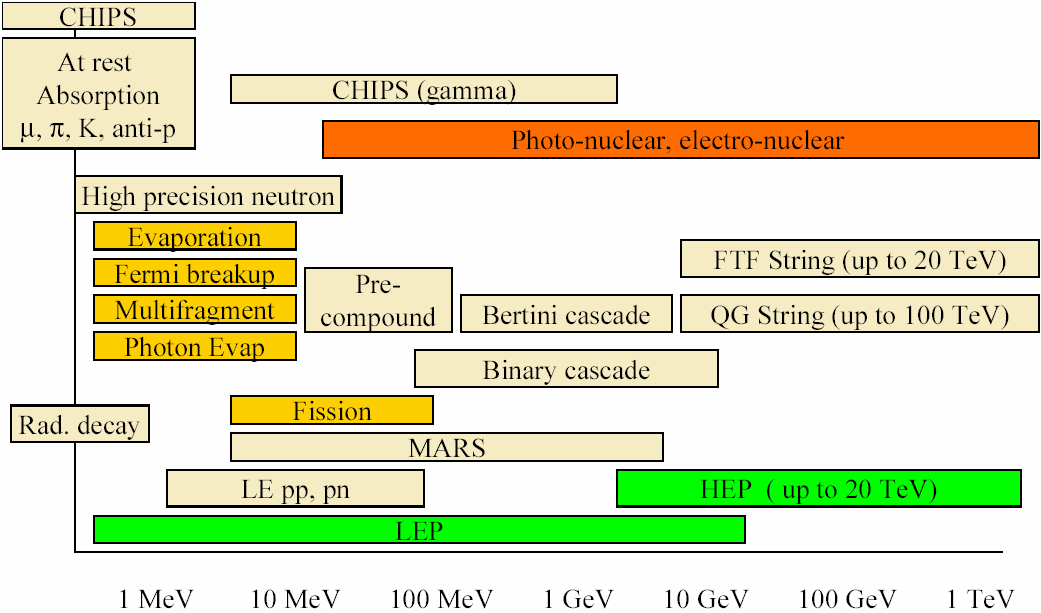
\includegraphics[width=.8\textwidth]{Digitizer/figs/HadronicModelsInventory.jpg}
    \caption{Les modèles utilisés dans GEANT4.}
    \label{fig.model}
  \end{center}
\end{figure}
\\
Les principaux modèles pour les interactions hadroniques de haute energie avec la matière sont les modèle de cordes partoniques (cf. section~\ref{sec.parton}) qui sont valables pour des énergies supérieur à $5-10$ GeV. Les intéractions aux énergies intermédiaires (100 MeV < E < 10 GeV) sont simulées avec les modèle de cascade intranucléaires (cf. section~\ref{sec.inucl}). Pour traiter les noyaux excités par des collisions de plus haute énergie et les intéractions en dessous de 200 MeV, une famille de modèle de désexcitation nucléaire (fission, évaporation nucléaire\dots) est disponible. Les intéractions des neutrons de basses énergies (E<20 MeV) peuvent être simulées avec des modèles de haute précision pour neutrons où un grand nombre de sections efficaces ont été tabulés. L'utilisation ou non de ces modèles de haute précision pour les neutrons aura des conséquences sur le temps de calcul, sur la réponse simulée du détecteur ou sur la topologie des gerbes\dots
\subsection{Modèles de cordes partoniques}
\label{sec.parton}
Les modèles de cordes partoniques permettent de simuler les réaction de hautes énergies de hadrons avec des noyaux. Les deux principaux modèles utilisés dans GEANT4 sont les modèles QGS (Quark Gluon String) et FTF (Fritiof) \cite{geant4_parton}. Le résultat de l'interaction d'un hadron avec un noyau est une ou plusieurs cordes excitées. Une corde est un segment où chacune des deux extrémités est un quark ou un di-quark se déplaçant dans des directions opposées. Les noyaux sont modèlisés comme un ensemble de nucléons dont les positions sont aléatoirement choisies en utimisant une distribution de densité. Pour les noyaux lourd (A>16), une distribution de densité de la forme du potentiel de Wood-Saxon est utilisée : 
\begin{equation}
  \rho(r_i)=\frac{\rho_0}{1+exp[(r_i-R)]/a}
\end{equation}
où $R$ et $a$ dépendent de la masse du noyau. Pour les noyau léger une distribution de densité venant du modèle d'oscillateur harmonique est utilisée : 
\begin{equation}
  \rho(r_i)=(\pi R'^2)^{-3/2}exp(-r_i^2/R'^2)
\end{equation}
avec $R'$  qui dépend de la masse du noyau.
Pour calculer le paramètre d'impact avec les nucléons, ces deux distribution de densité sont réduites dans un plan perpendiculaire à la direction de la particule incidente. La probabilité de collision entre entre le hadron et un nucléon est calculée en utilisant une distribution gaussienne pour les fonctions d'onde du hadron et des nucléons. Ces probabilités sont utilisée pour connaitre le nombre de nucléons participant à la réaction dans le noyau.\\
Des cordes sont ensuites crées, les quarks du hadron incident sont aléatoirement répartis entre celles-ci. Un modèle de fragmentation longitudinal de cordes est ensuite utilisé où ces cordes sont séparées en hadrons et en une nouvelle corde. Une corde se fragmente en une paire quark-antiquark $q-\bar q$ ou diquark-antidiquark $qq-\bar q \bar q$ \cite{geant4_reference}. Les probabilités relatives de création des quark ou diquark sont :
\begin{equation}
  u:d:s:qq = 1:1:0.35:0.1
\end{equation}
La paire de quark-antiquark (ou diquark-antidiquark) créée est placée entre la précédente paire. Une moitié de ces nouvelles paires sont utilisées pour créer un hadron tandis que les autres constituants créent une nouvelle corde. Ce processus se répète jusqu'à ce que l'énergie d'une corde ne soit pas suffisante pour créer un hadron.\\
Après l'interaction du noyau avec la particule incidente, celui-ci sera dans un état excité. Le retour à l'état fondamental du noyau est simulée avec des modèle de fragmentation, précomposé et de désexcitation nucléaire.
\begin{table}[!ht]
  \begin{center}
    \begin{tabular}{c|c|c}
      Particule & QGS & FTF\\
      \hline
      $k+$ & $12\ GeV\ -\ 100\ TeV$ & $4\ GeV\ -\ 100\ TeV$\\
      $k-$ & $12\ GeV\ -\ 100\ TeV$ & $4\ GeV\ -\ 100\ TeV$\\
      $\lambda$ & $ $ & $2\ GeV\ -\ 100\ TeV$\\
      $\pi+$ & $12\ GeV\ -\ 100\ TeV$ & $4\ GeV\ -\ 100\ TeV$\\
      $\pi-$ & $12\ GeV\ -\ 100\ TeV$ & $4\ GeV\ -\ 100\ TeV$\\
      $neutron$ & $12\ GeV\ -\ 100\ TeV$ & $4\ GeV\ -\ 100\ TeV$\\
      $proton$ & $12\ GeV\ -\ 100\ TeV$ & $4\ GeV\ -\ 100\ TeV$\\
      $ion$ & $ $ & $2\ GeV\ -\ 100\ TeV$\\
    \end{tabular}
  \end{center}
  \caption{Chambers list where threshold are changed.}
  \label{tab.partonModelTable}
\end{table}
\subsection{Le modèles de cascade intranucléaire de Bertini}
\label{sec.inucl}
Il a été montré dans \cite{bertini} en 1969 qu'un modèle de cascade intranucléaire décrivait relativement bien les intéractions de nucléons de 100 MeV à 2 GeV avec des noyaux. Ces réactions sont caractérisées par une rapide ($10^{-23}-10^{-22} s$) cascade intranucléaire laissant les noyaux dans un état excité, suivi d'une phase plus lente ($10^{-18}-10^{-16} s$) d'évaporation nucléaire. blabblba geant4 deux modèle...
\begin{figure}[!ht]
  \begin{center}
    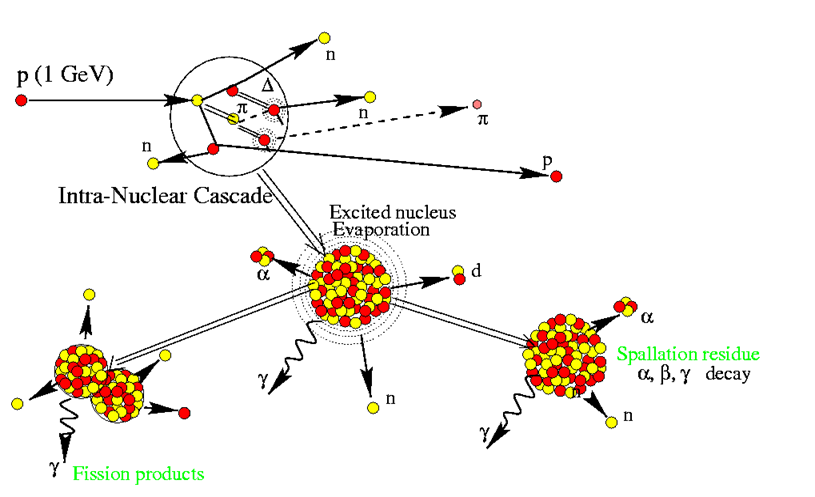
\includegraphics[width=.8\textwidth]{Digitizer/figs/intraNucl.png}
    \caption{Schéma d'explication du modèle de Bertini. Un hadron de 400 MeV crée une cascade intraucléaire.}
    \label{fig.g4bertini}
  \end{center}
\end{figure}
\subsubsection{Bertini}
Ce modèle a depuis été étendu et est valable pour des particules incidentes ($p,n,\pi,K,\Delta,\Sigma,\Xi,\Omega$ et $\gamma$) avec une énergie cinétique comprise entre 100 MeV et 10 GeV~\cite{geant4_bertini}. Ce modèle est applicable lorsque la longueur d'onde de deBroglie de la particule incidente est de l'ordre de la distance moyenne entre les nucléons du noyau. Le noyau cible est modèlisé par jusqu'à six couche concentrique de densité constate. La cascade commence lorsque une particule incidente rencontre un nucléon du noyau cible et produit des particules secondaires. Ces particules secondaires intéragissent alors avec les autres nucléons, sont absorbés ou s'échappent du noyau. La cascade prend fin lorsque toutes les particules secondaires sont soit absorbées soit se sont échappées. La figure~\ref{fig.g4bertini} illustre le phénomène de cascade intranucléaire.
\subsubsection{Binary}
Dans GEANT4, un autre modèle de cascade intranucléaire est disponible et est utilisé par certaine liste physique. C'est le modèle de cascade binaire. 
\subsection{Les listes physiques}
\label{sec.listphys}
\begin{figure}[!ht]
  \begin{center}
    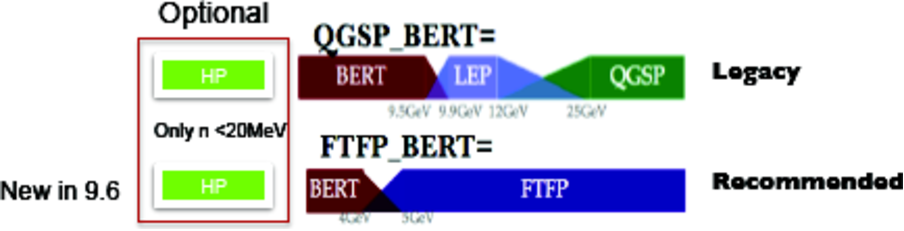
\includegraphics[width=.8\textwidth]{Digitizer/figs/physics_list_G4.pdf}
    \caption{Liste physique.}
    \label{fig.g4list}
  \end{center}
\end{figure}

%%%%%%%%%%%%%%%%%%%%%%%%%%%%%%%%%%%%%%%%%%%%%%%

\section{La simulation du prototype}
La simulation du prototype SDHCAL a été réalisé avec un programme basé sur GEANT4 \cite{geant4}. La géométrie du détecteur est décrite dans ce programme avec de nombreux détails. Les compositions chimiques, les densités des matériaux du prototypes sont utilisés. Ces informations seront utilisées par GEANT4 pour des calculs de sections efficaces lors de la propagation des particules dans le détecteur. Le champ électrique entre les deux électrodes de verre des GRPC n'est pas simulé. Les avalanches issues des ionisations du gaz par les particules incidentes sont modélisés par un algorithm dédié qui sera décrit dans la partie \ref{sec.digit-algo} de ce chapitre. La trajectoire des particules primaires et secondaires est segmentée dans GEANT4. A chaque intéraction avec les matériaux du détecteur un nouveau segment est créé. La création d'un nouveau segment se fait aussi à chaque fois qu'une particule change de volume (e.g. passant du verre au gaz). La liste des segments se trouvant dans le milieu actif du détecteur (le gaz entre les électrodes pour le SDHCAL) est alors enregistrée. Les informations stockées pour ces segments sont les suivantes: les coordonnées des positions du début et de la fin du segment; l'énergie perdue par la particule le long du segment; la nature de la particule; le temps d'occurence du segment relatif au moment où la particule primaire a été générée. 
Cette liste de segment est ensuite utilisé comme point de départ de l'algorithm utilisé pour modéliser la reponse des GRPC au particules chargées.

%%%%%%%%%%%%%%%%%%%%%%%%%%%%%%%%%%%%%%%%%%%%%%%

\section{Modèlisation de la réponse des GRPC au particules chargées}
Nous venons de voir que le résultat du programme de simulation du SDHCAL est une liste de segments correspondant à une partie ed la trajectoire d'une particule dans le détecteur. Nous avons vu que l'énergie déposée par ces segments étaient disponible alors que dans le cas du SDHCAL la charge induite sur les carreaux de cuivre est mesurée. De plus, le phénomène de multiplicité introduit au chapitre \ref{chap.sdhcal} n'est pas pris en compte par GEANT4. 
\label{sec.digit-algo}
%%%%%%%%%%%%%%%%%%%%%%%%%%%%%%%%%%%%%

\subsection{Algorithme SimDigital}
La modélisation est faite à l'aide d'un algorithm appelé SimDigital qui est un processeur Marlin \cite{marlin} disponible dans le paquet MarlinReco \cite{marlinreco} de l'ILCSoft \cite{ilcsoft}. Le but de cet algorithm est de simuler la charge induite par le passage d'une particule chargée dans le gaz, de distribuer cette charge sur les canaux de lecture et enfin d'appliquer les seuils. Les différentes étapes de l'algorithm sont les suivantes:
\begin{enumerate}[~~1-]
\item La fenêtre en temps utilisée dans la procédure de reconstruction des évenements décrites dans la partie \ref{sec.trivent} du chapitre \ref{chap.sdhcal} est de 1000 $ns$. Ainsi, les particules interragissant tardivement dans le détecteur comme les neutrons peuvent ne pas être associées à l'évenement. Pour prendre cet effet en compte, les segments avec un temps d'occurence supérieur à 1000 $ns$ sont supprimée.
\item \label{it.start} Un canal de lecture $C_0$ où un ou plusieurs segments ont traversé le gaz est sélectionné. La longueur de ses segments est alors calculée.
\item La longueur de certains des segments dans le gaz peut être très petite. Ce phénomène peut arriver aléatoirement lors de la propagation des particules par GEANT4. Cependant la majorité des cas où ce phénomène s'observe, s'explique par le changement de volume d'une particule. La figure~\ref{fig.map_and_length_vs_deltaz}(a) présente la longueur des segments en fonction de $\Delta_z$ où $\Delta_z$ correspond à la distance entre la position du milieu du segment et le milieu de la couche de gaz. Cette figure montre qu'une grande fraction des segments de faible longueur sont proches des deux électrodes en verre ($|\Delta_z|\simeq0.6$).
  \begin{figure}[!ht]
    \subfigure[]{\includegraphics[width=0.5\textwidth]{Digitizer/figs/sstepLength_vs_deltaZ_ZOOM.pdf}}
    \subfigure[]{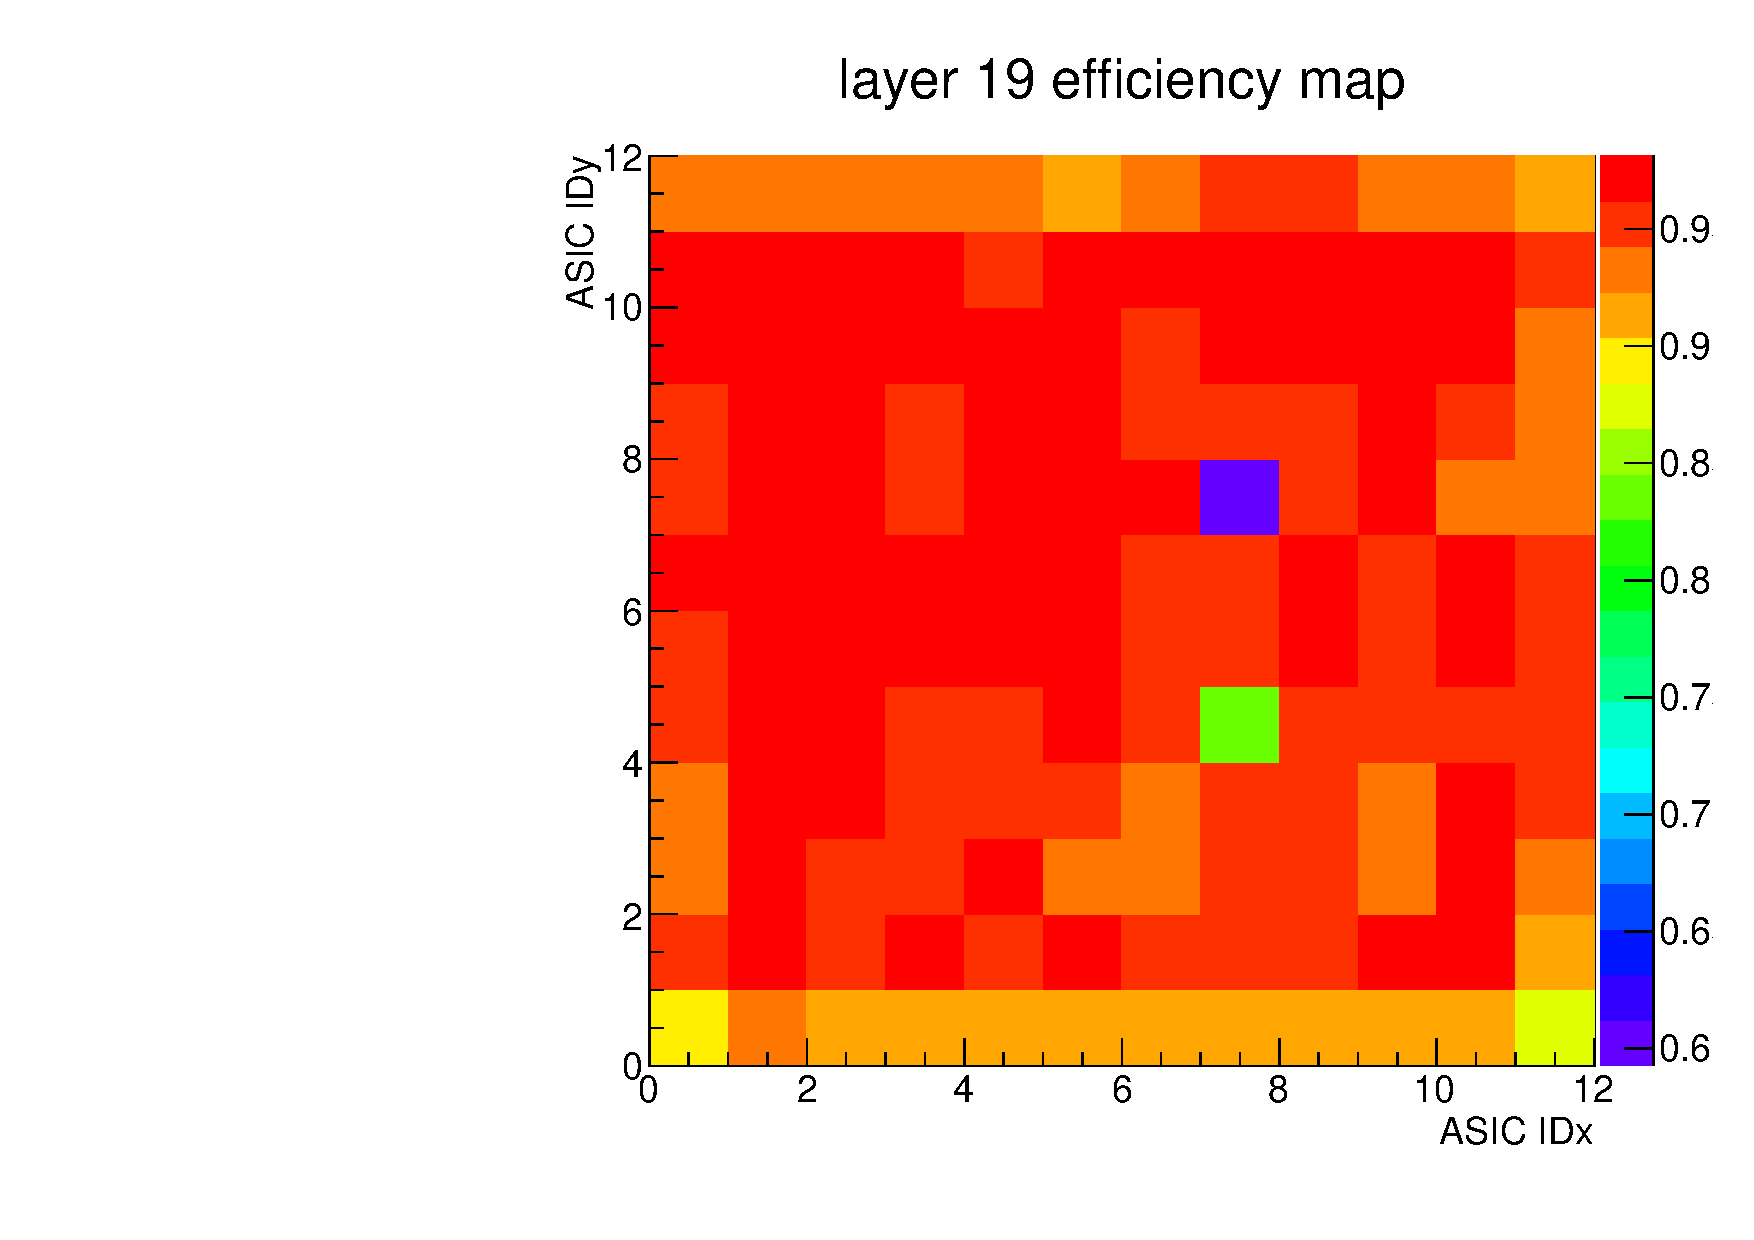
\includegraphics[width=0.5\textwidth]{Digitizer/figs/layer19map.pdf}}
    \caption{(a): Longueur des segments en $mm$ en fonction de $\Delta_z$ en $mm$. Cette figure est centrée sur la région des segments de faible longueur pour mettre en évidence le fait que la plupart des segmets de longueur nulle (ou presque) sont localisé sur les bords de la couche de gaz ($|\Delta_z|\simeq0.6\ mm$). (b): Exemple d'une carte d'efficacité des ASICs.}
    \label{fig.map_and_length_vs_deltaz}
  \end{figure}
\item Les cartes d'efficacité des ASIC du prototype déterminés grace à l'étude des muons décrite dans la partie \ref{sec.muons} du chapitre \ref{chap.sdhcal}, sont utilisées pour prendre en compte les effets des $quenchers$ ($CO_2$,$SF_6$). En effet, les propriétés de ces deux gaz (capture des photons et d'électrons) ne sont pas incluses dans GEANT4. De plus, l'utilisation de ces cartes d'efficiacité permet d'éviter la présence de signal dans les canaux électroniques hors d'usage ou masqués. Ainsi, lorsqu'un segment est dans une région du détecteur où l'efficacité est de 50\% alors ce segment a 50\% de chance d'être conservé. La figure \ref{fig.map_and_length_vs_deltaz} montre un exemple de carte d'efficacité d'une chambre du prototype SDHCAL.
\item La charge induite pour chaque segment est alors aléoiterement choisis dans une distribution de Polya: 
  \begin{equation}
    \label{eq.polya}
    P(q)=[\frac{q}{\bar q}(1+\theta)]^{\theta}e^{[-\frac{q}{\bar q}(1+\theta)]}
  \end{equation}
  où $\bar q$ est la valeur moyenne et $\theta$ un paramètre libre lié à la largeur de la distribution. Cette charge innduite est ensuite corrigée: 
  \begin{equation}
    \label{eq.lengthcorrection}
    Q_{corr} = \left\{ \begin{array}{rl}
      Q_{ind}(\frac{d_s}{d_{gap}})^\kappa &\mbox{ si $\frac{d_s}{d_{gap}}>1$} \\
      Q_{ind} &\mbox{ sinon}
    \end{array} \right.
  \end{equation}
  où $d_s$ correspond à la longueur du segment, $d_{gap}$ à l'épaisseur de la couche de gaz (1.2 $mm$) et $\kappa$ un paramètre libre. L'effet et l'importance de cette correction sera discuté dans la partie \ref{sec.param} de ce chapitre.
\item Dans les gerbes hadroniques et électromagnétiques, les particules chargés peuvent être très proches. Ainsi les avalanche induites dans le gaz par ces particules peuvent se chevaucher. Cependant, dans le régime avalanche le signal induit par ces particules n'est pas équivalent à la somme des signaux induits par ces particules pris individuellement. Pour simuler cet effet, lorsque la distance entre deux segments est inférieure à une valeur $d_{cut}$, le segment dont la charge induite ($Q_{corr}$) est la plus faible, est supprimé. Ce filtre permet aussi de supprimer un ou plusieurs segments provenant d'une seule particule. En effet, une intéraction entre une particule chargée et le gaz peut avoir lieu dans GEANT4. Ainsi plusieurs segments seraient créés et pourraient déclencher une avalanche alors qu'une seule particule est passée.
\item La charge induite est ensuite réparti sur le canal de lecture $C_0$  et sur les canaux voisins. Les canaux voisins correspondent au cellules dans le même plan que $C_0$ à une distance inférieur à une valeur $r_{max}$. Un rapport est alors calculé pour chaque canal:
  \begin{equation}
    \label{eq.ratio}
    R_i = \frac{\int_{a_i}^{b_i}\int_{c_i}^{d_i}\sum_{j=0}^{n}\alpha_j e^{ \frac{(x_0-x)^2+(y_0-y)^2}{\sigma_j^2}}dxdy}{N}
  \end{equation}
  où $a_i,\ b_i,\ c_i,\ d_i$ sont les positions des bords de la cellule $i$, $(x_0,y_0)$ sont les coordonneés du milieu du segment et N un facteur de normalisation définit comme: 
  \begin{equation}
    \label{eq.norm}
    N=\int_{-r_{max}}^{+r_{max}}\int_{-r_{max}}^{+r_{max}}\sum_{j=0}^{n}\alpha_j e^{ \frac{(x_0-x)^2+(y_0-y)^2}{\sigma_j^2}}dxdy
  \end{equation}
\item Pour chaque canal ($C_0$ et ses voisins), un paramètre de charge est augmenté d'une valeur $R_iQ_{corr}$.
\item L'opération est répétée à partir de l'étape \ref{it.start} pour tous les canaux avec des segments.
\item Les seuils sont finalement appliqués pour tous les canaux.
\end{enumerate}

%%%%%%%%%%%%%%%%%%%%%%%%%%%%%%%%%%%%%

\subsection{Paramétrisation de l'algorithme}
\label{sec.param}
%%%%%%%%%%%%%%%%%%%%%%%%%%%%%%%%%%%%%

\subsubsection{Mesure du spectre de charge}

\begin{figure}[!ht]
  \subfigure[]{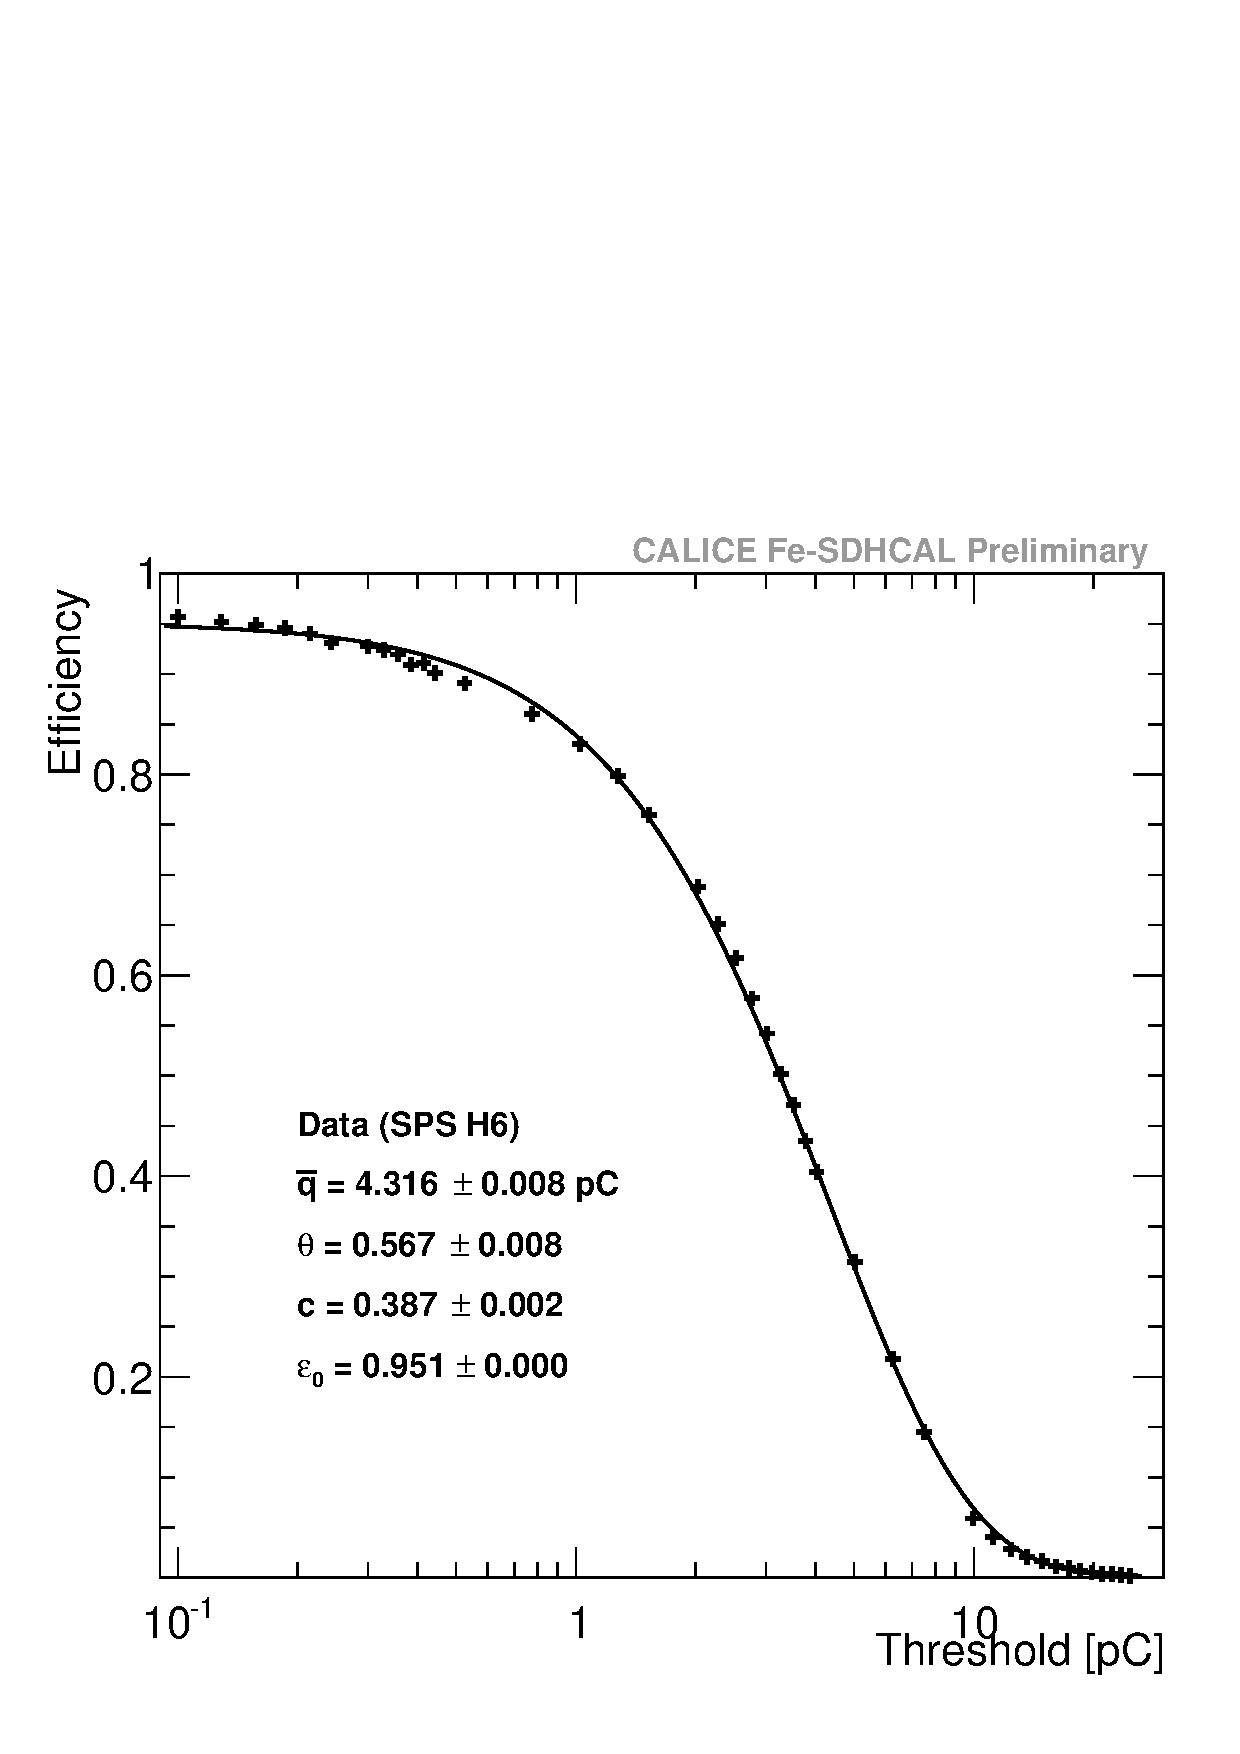
\includegraphics[width=.5\textwidth]{Digitizer/figs/thrScanDat.pdf}}
  \subfigure[]{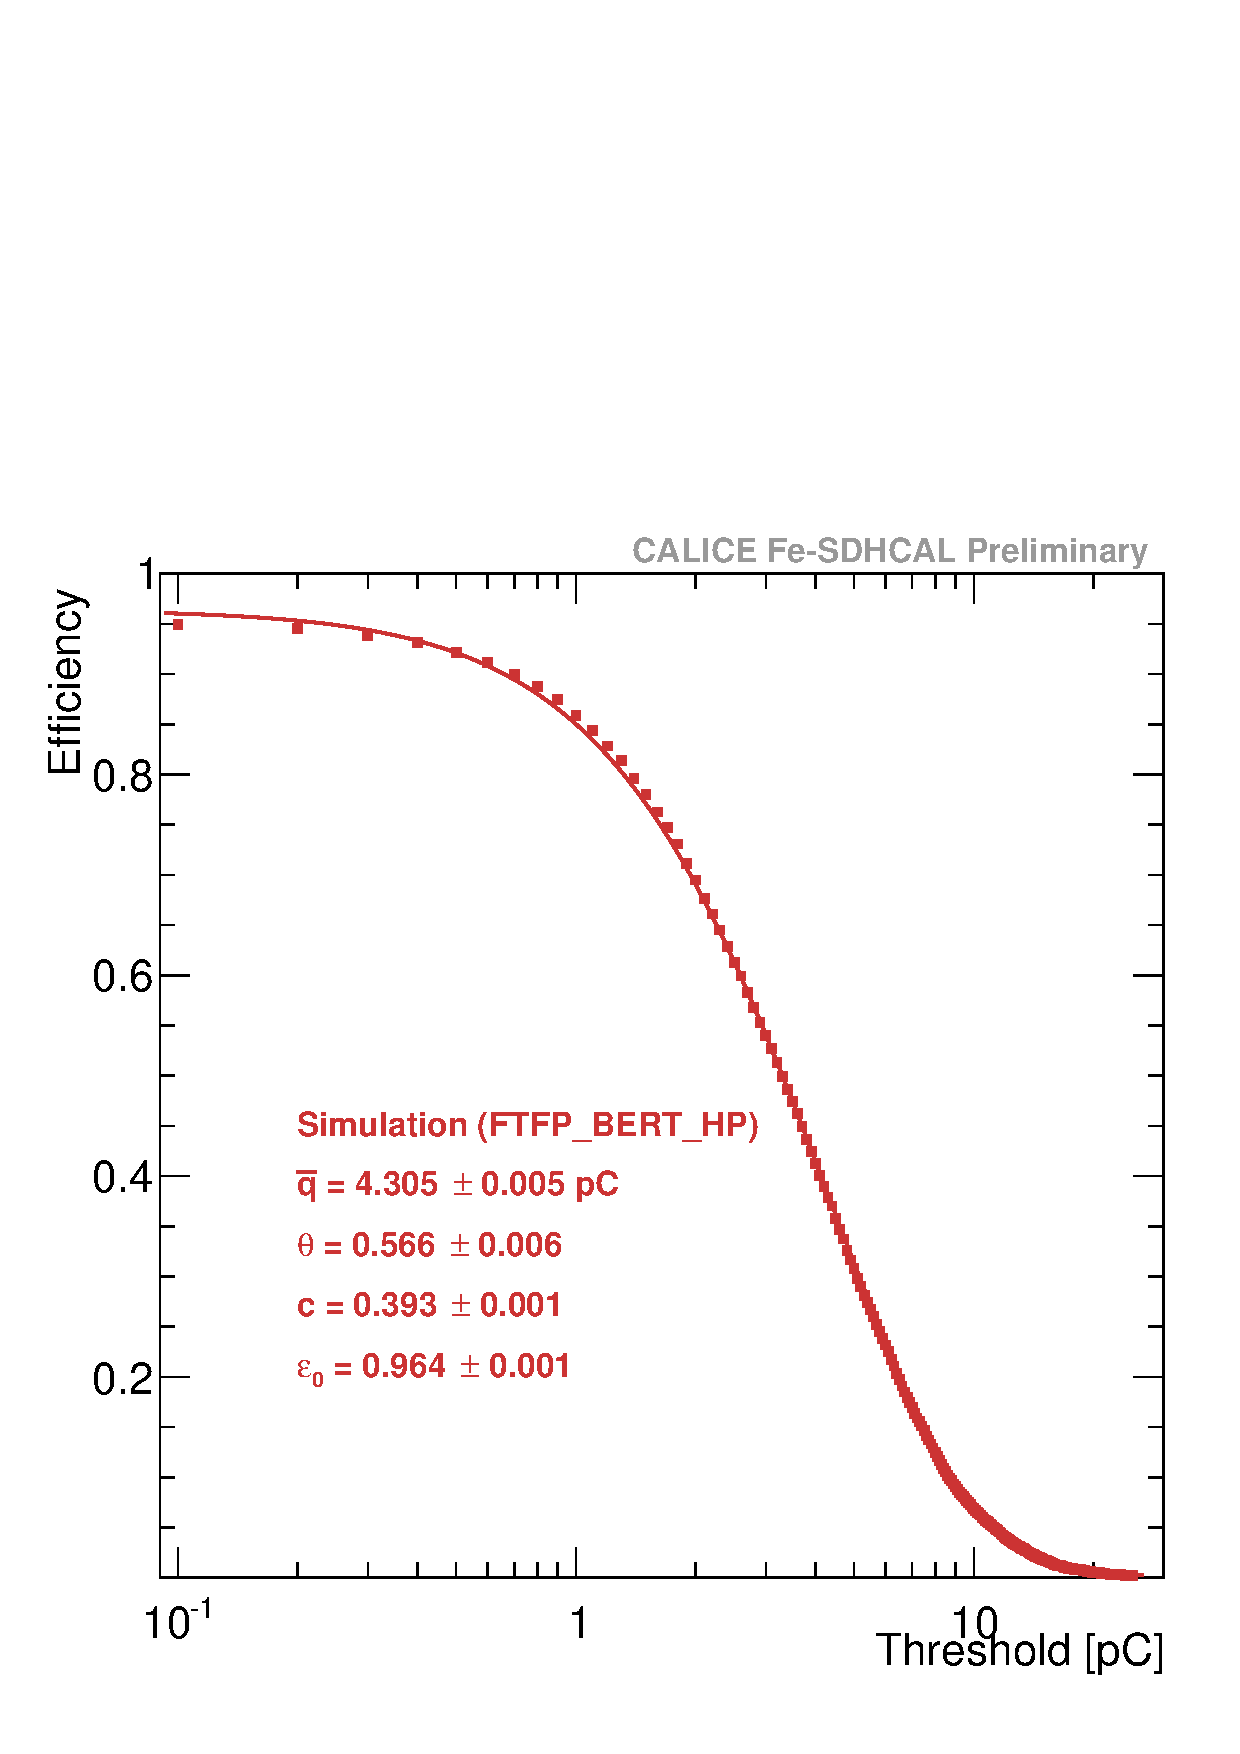
\includegraphics[width=.5\textwidth]{Digitizer/figs/thrScanSim.pdf}}
  \caption{(a) Résultats du scan en seuil pour les données (a) et pour la simulation (b). \label{fig.thrScan}}
\end{figure}

%%%%%%%%%%%%%%%%%%%%%%%%%%%%%%%%%%%%%

\subsubsection{Répartition de la charge}

\begin{figure}[!ht]
  \subfigure[]{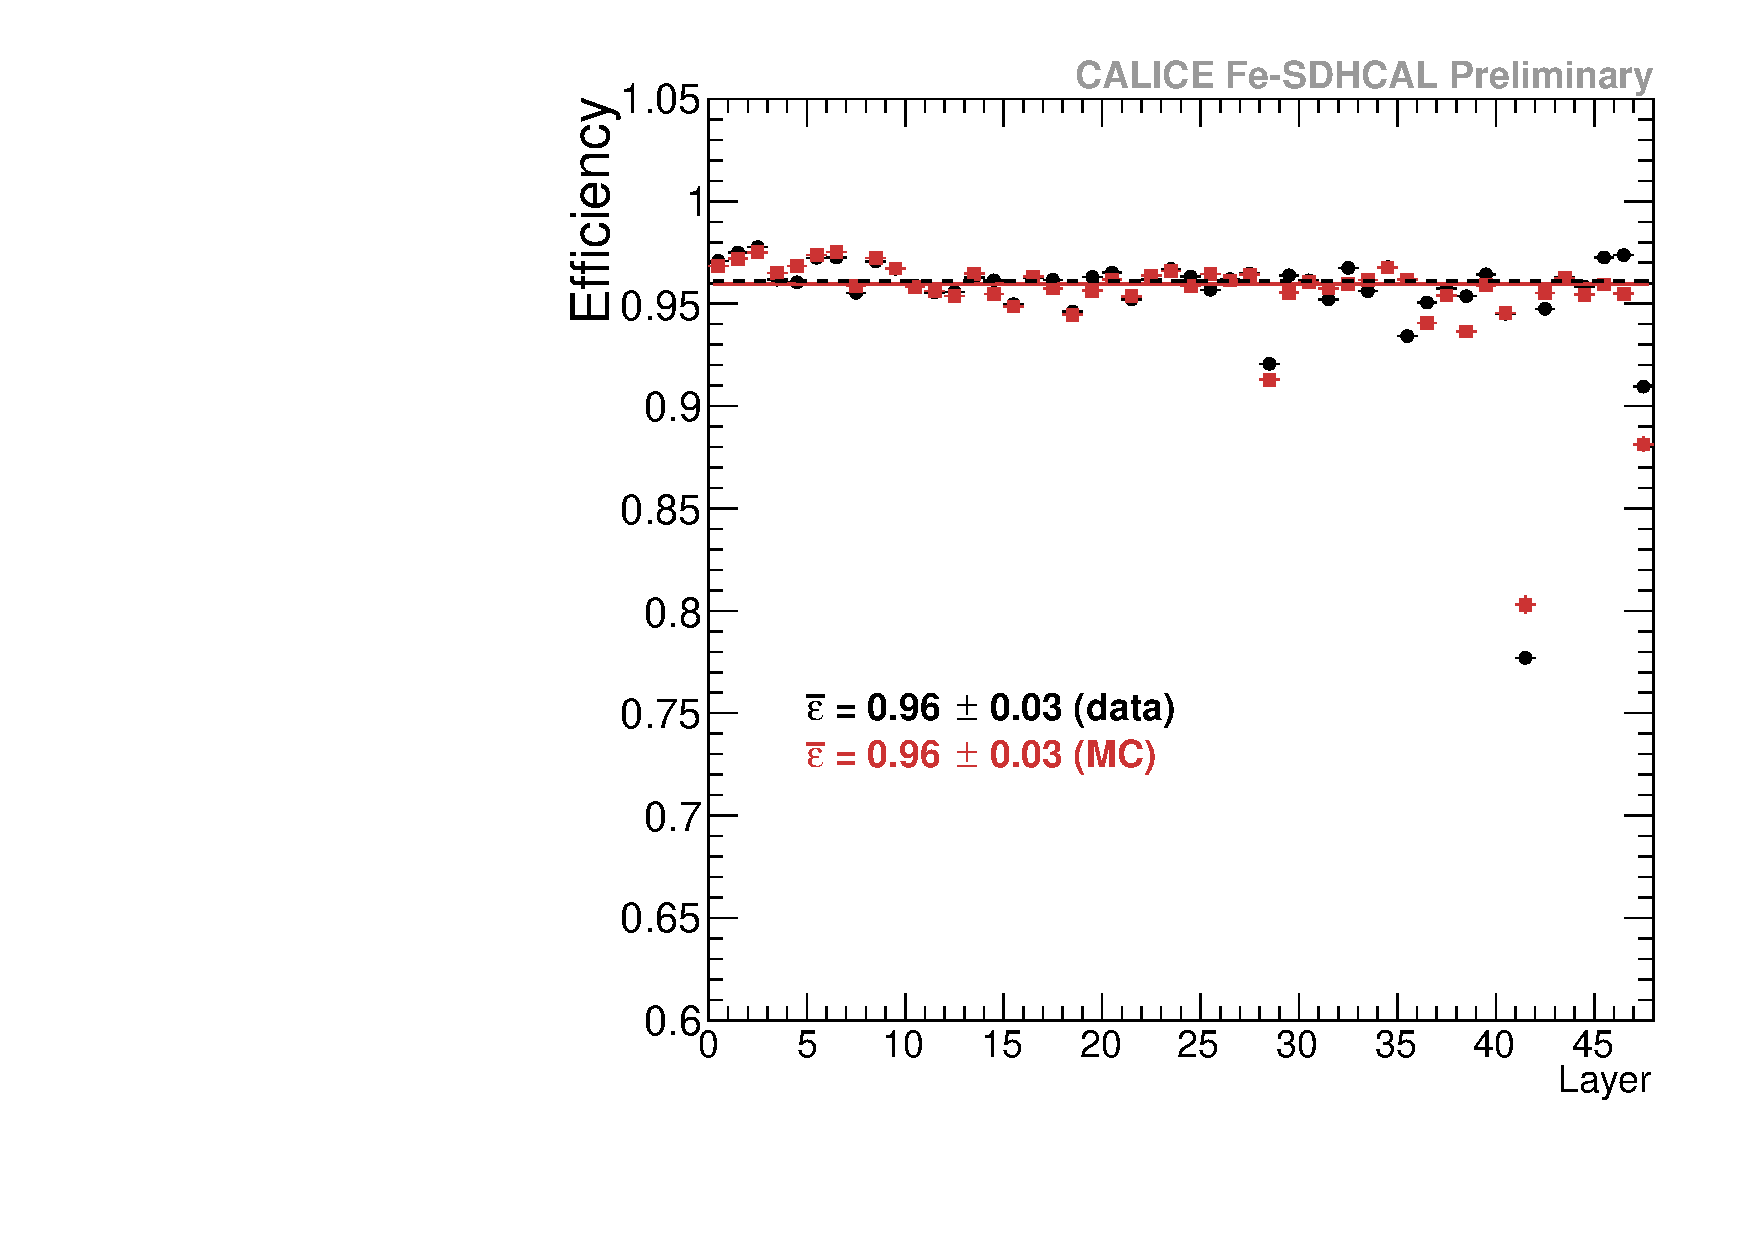
\includegraphics[width=.5\textwidth]{Digitizer/figs/effLayer.pdf}}
  \subfigure[]{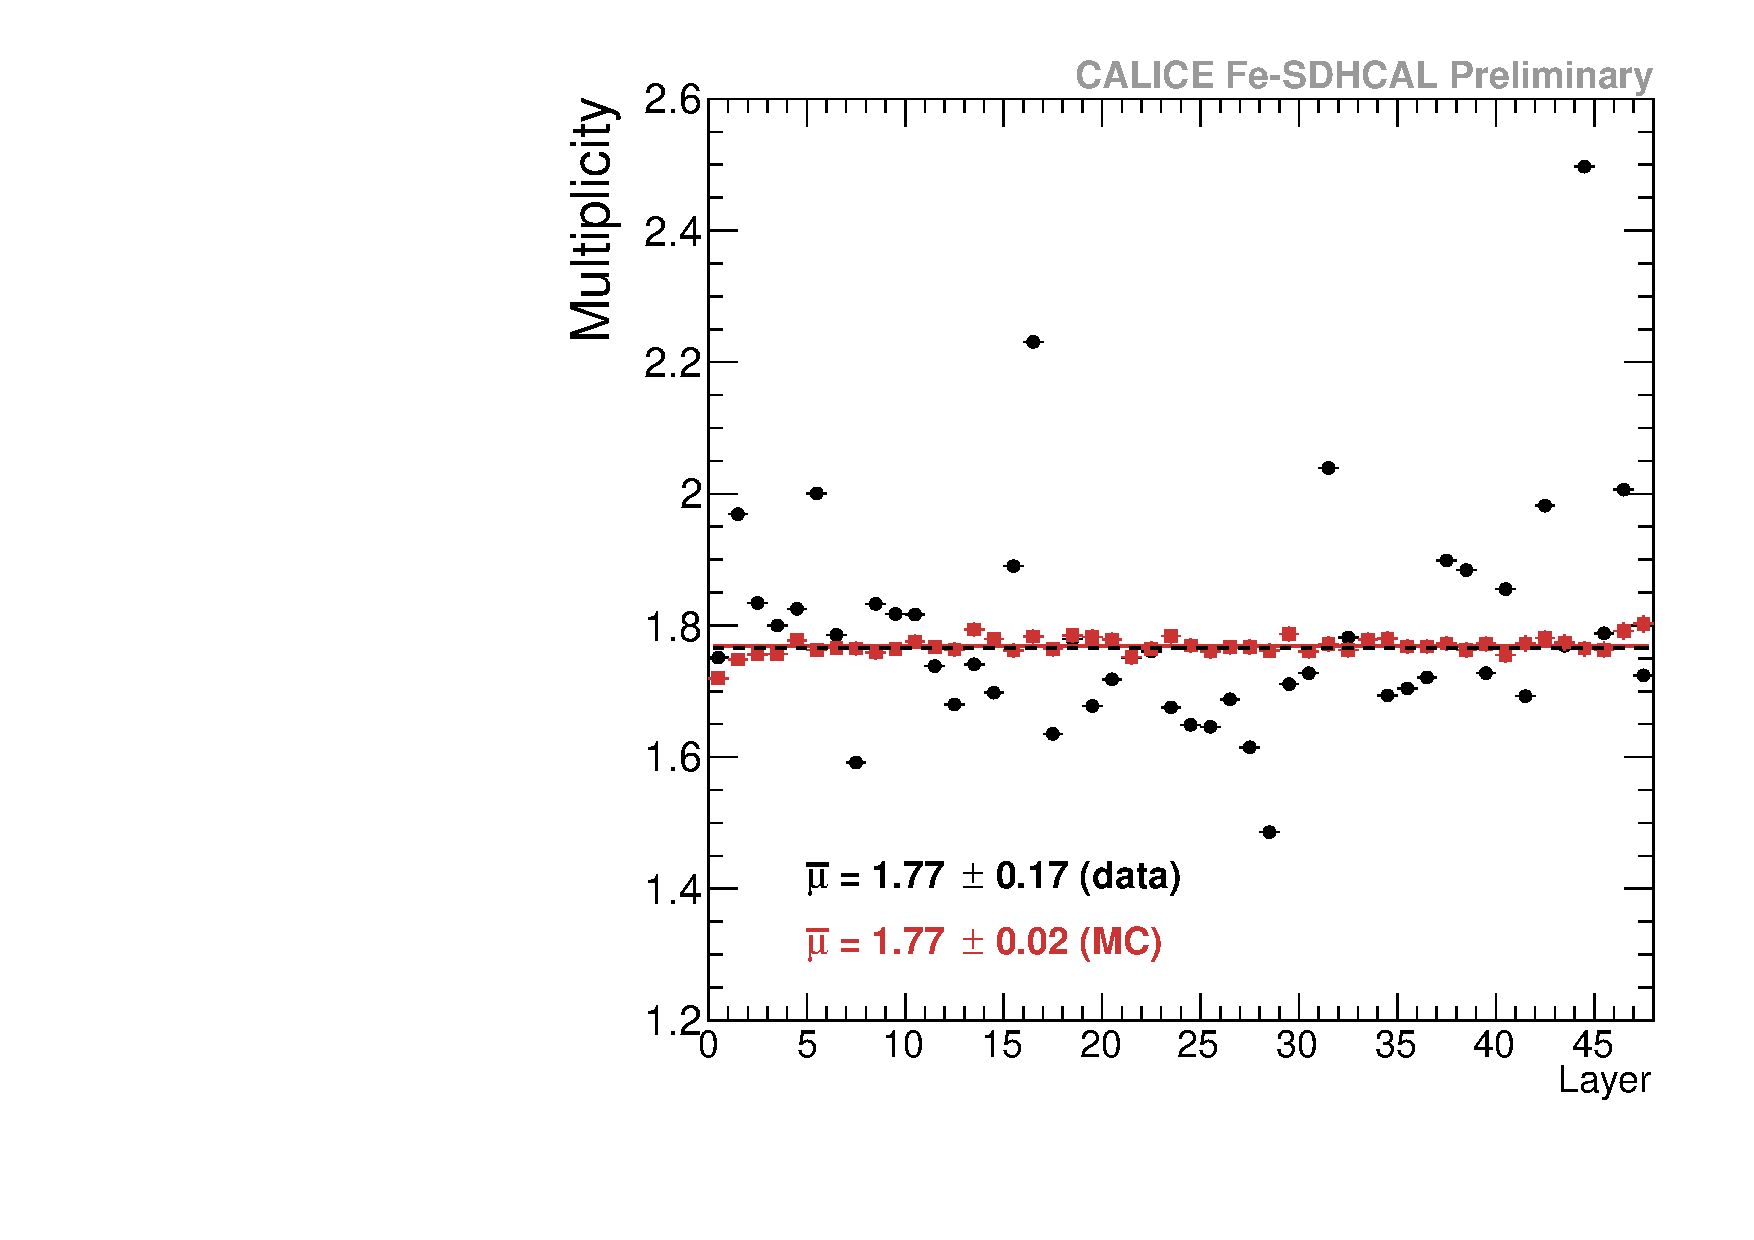
\includegraphics[width=.5\textwidth]{Digitizer/figs/mulLayer.pdf}}
  \caption{Efficacité (a) et multiplicité (b) par plan. Les données sont représentées par des cercles noirs et la simulation par des carrés rouges.\label{fig.eff_mul_layer}}
\end{figure}

%%%%%%%%%%%%%%%%%%%%%%%%%%%%%%%%%%%%%

\subsubsection{Dépendance de l'angle d'incidence}

\begin{figure}[!ht]
  \begin{center}
    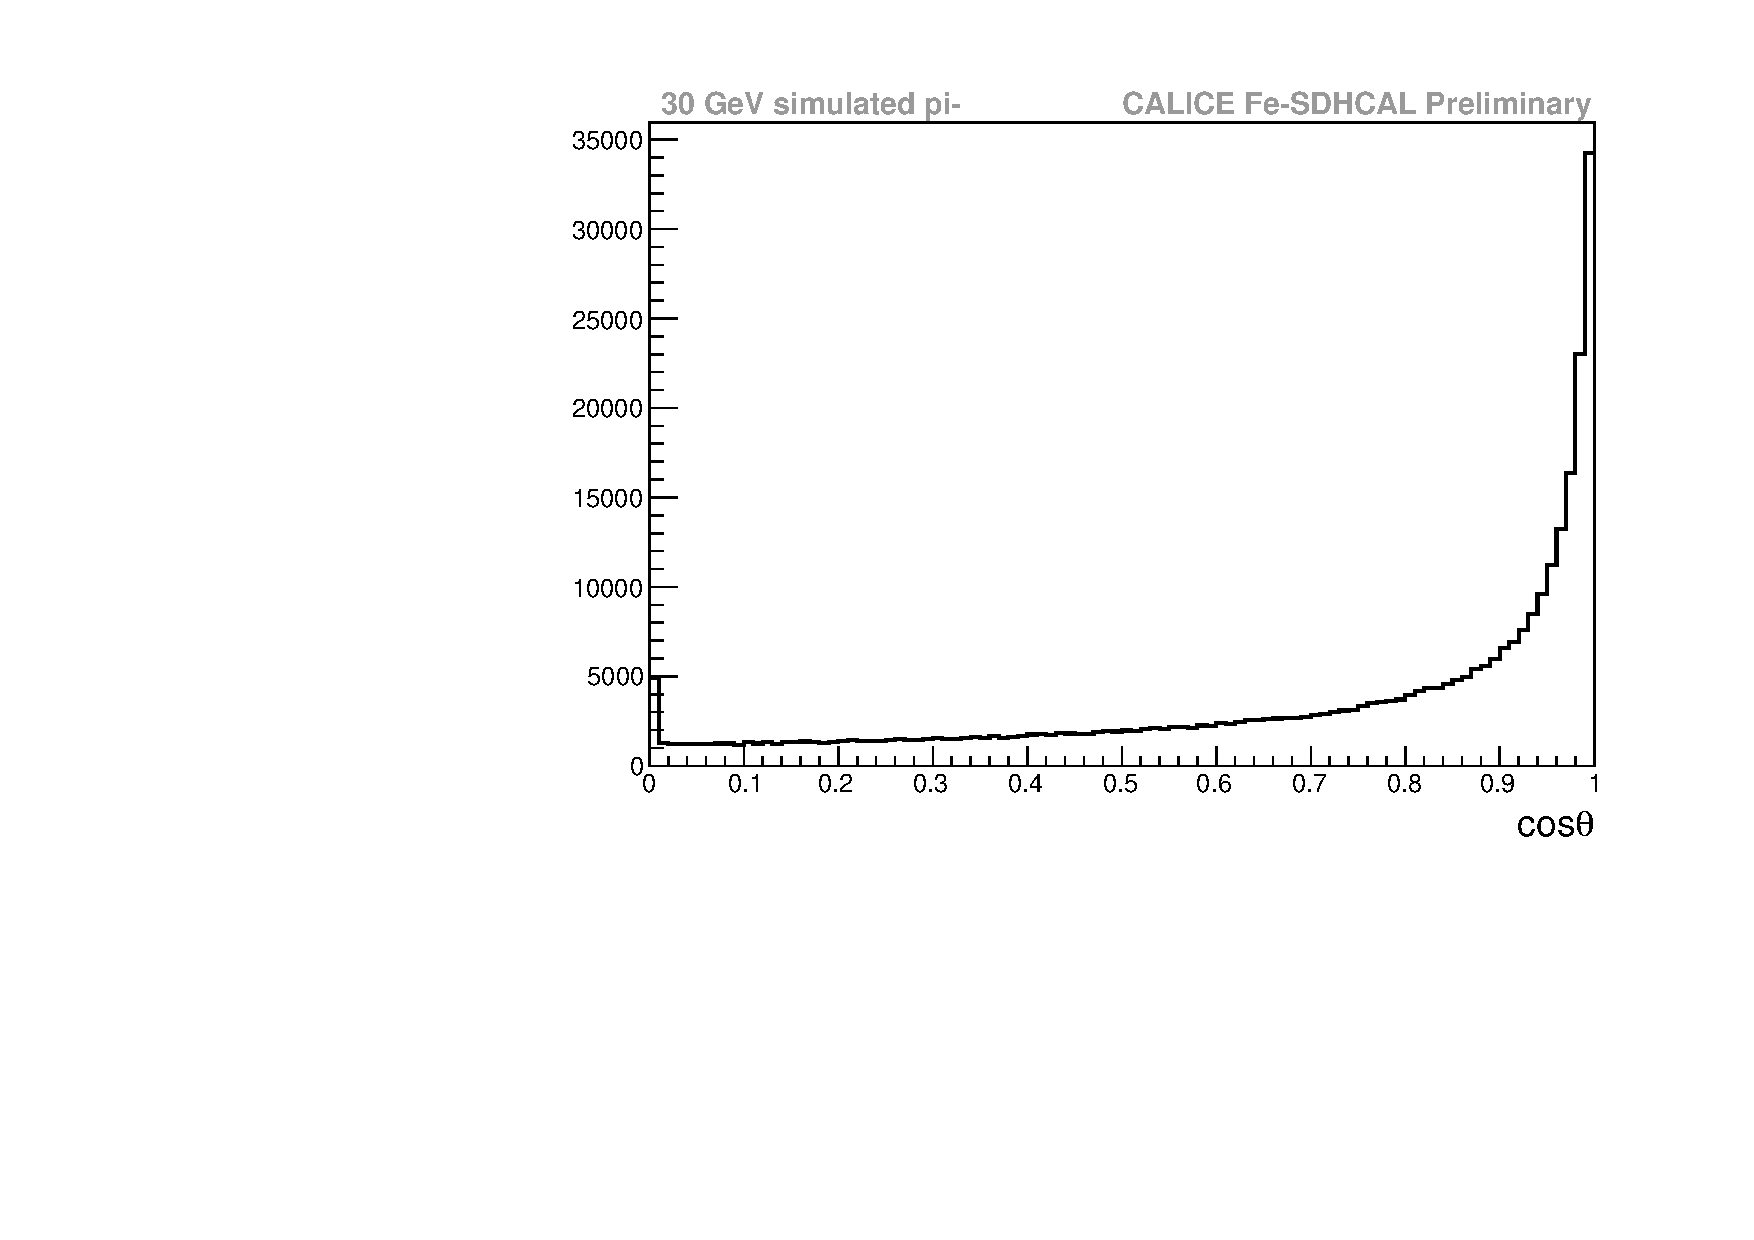
\includegraphics[width=.8\textwidth]{Digitizer/figs/costhetaPI30.pdf}
    \caption{Distribution du cos de l'angle de la step avec la normal à la GRPC pour une simulation d'un échantillon de pion à 30 GeV.}
    \label{fig.g4list}
  \end{center}
\end{figure}

\begin{figure}[!ht]
  \subfigure[]{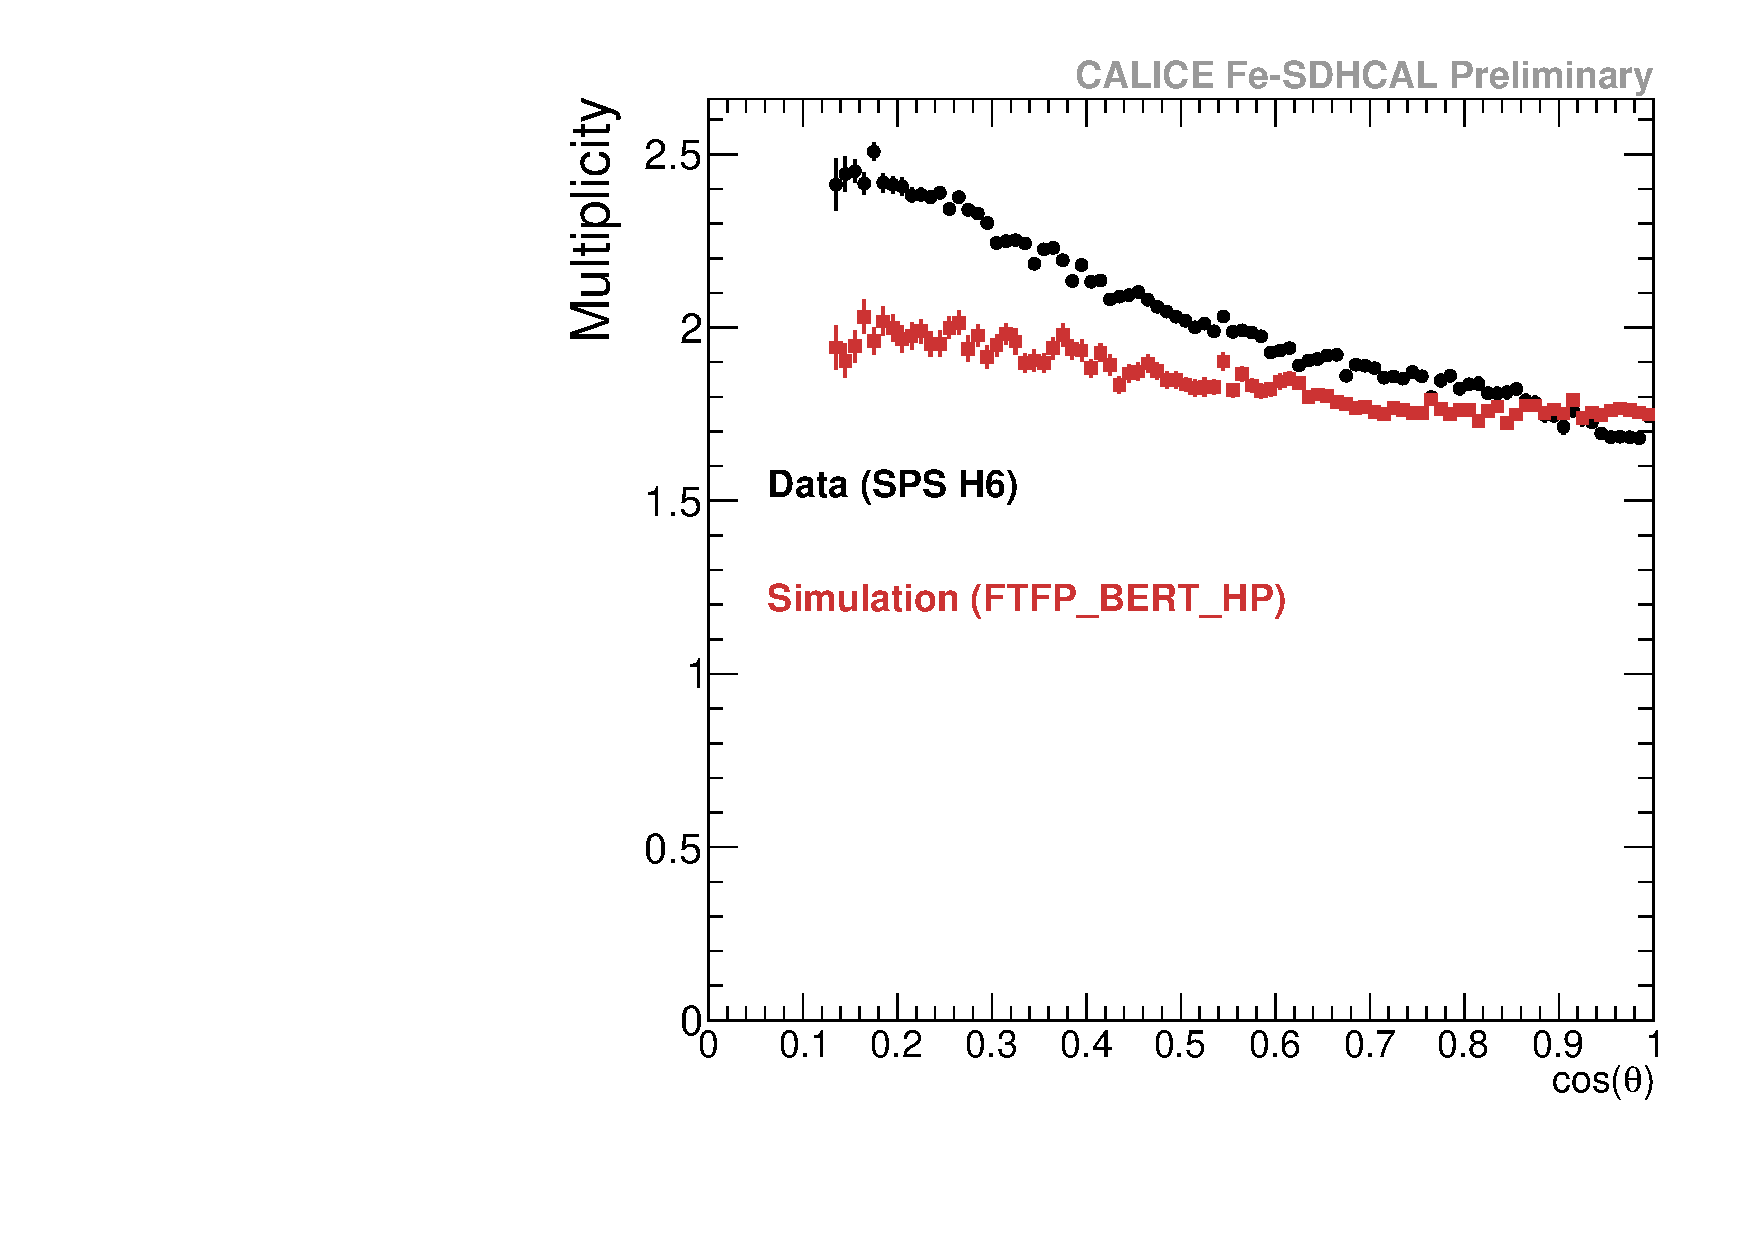
\includegraphics[width=.5\textwidth]{Digitizer/figs/mul_vs_thetaNLC.pdf}}
  \subfigure[]{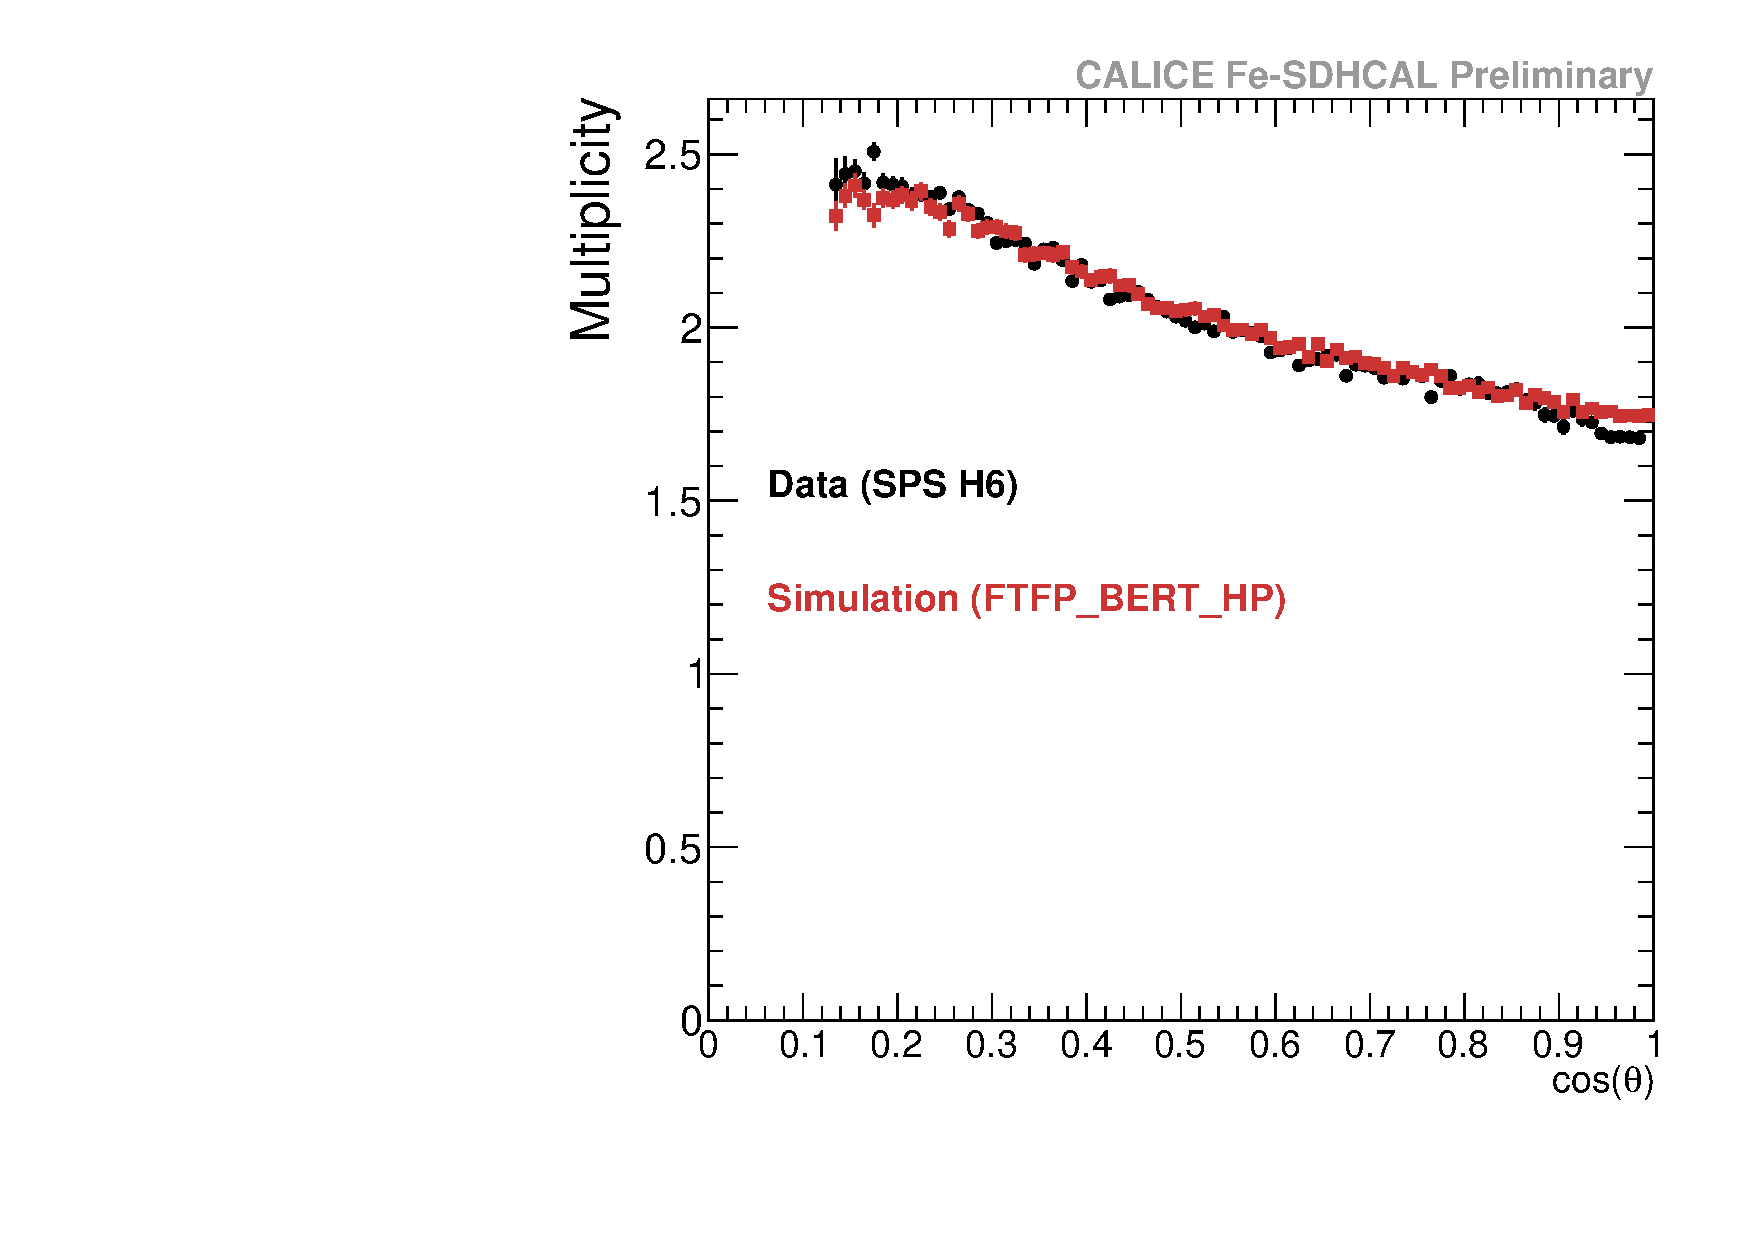
\includegraphics[width=.5\textwidth]{Digitizer/figs/mul_vs_theta.pdf}}
  \caption{Multiplicité moyenne en fonction de $cos\theta$ avec des cercles noirs et des carré rouges pour les données et la simulation respectivement. (a): sans correction sur la longueur des steps; (b) avec correction sur la longueur des steps. \label{fig.eff_mul_layer}}
\end{figure}

%%%%%%%%%%%%%%%%%%%%%%%%%%%%%%%%%%%%%

\subsection{Résultats}

%%%%%%%%%%%%%%%%%%%%%

\subsubsection{Gerbes électromagnétique}
\begin{figure}[!ht]
  \subfigure[]{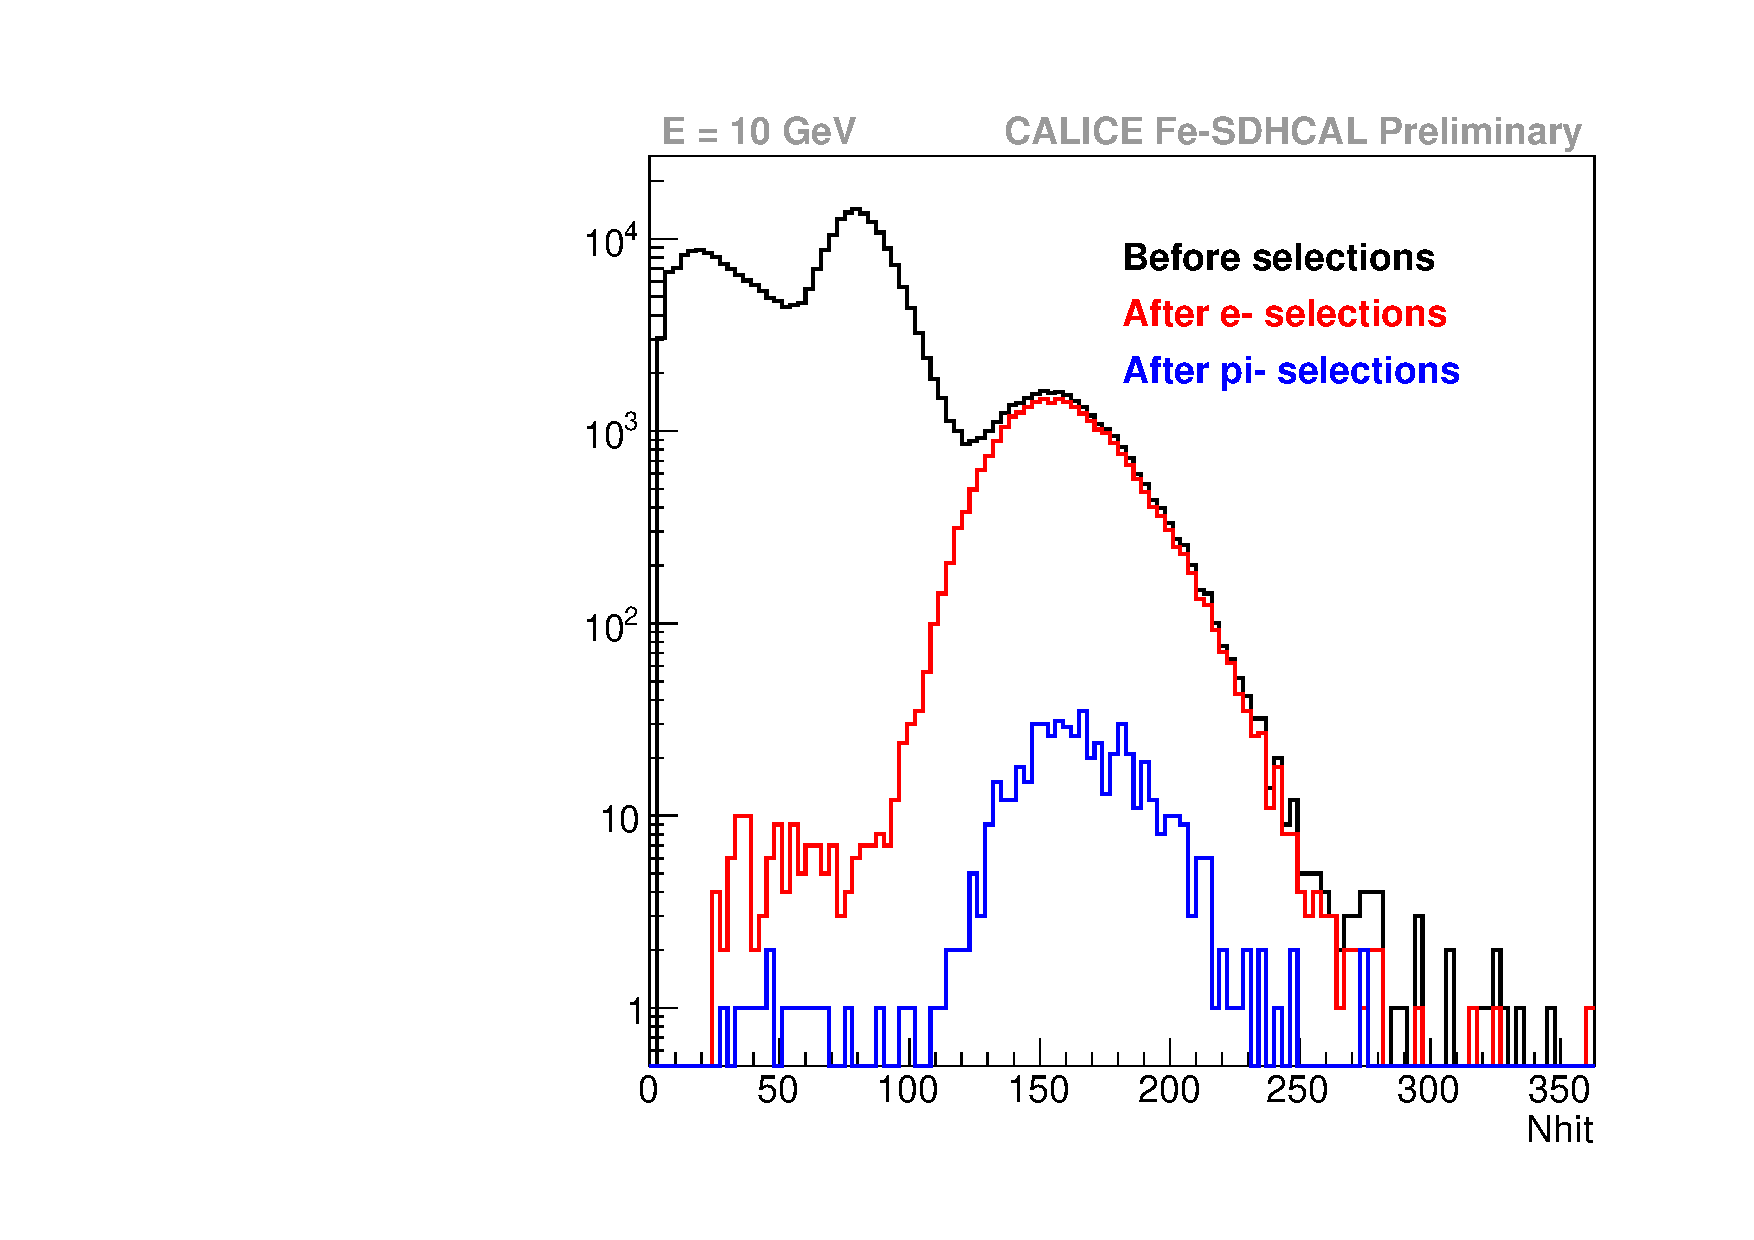
\includegraphics[width=.5\textwidth]{Digitizer/figs/selection715725.pdf}}
  \subfigure[]{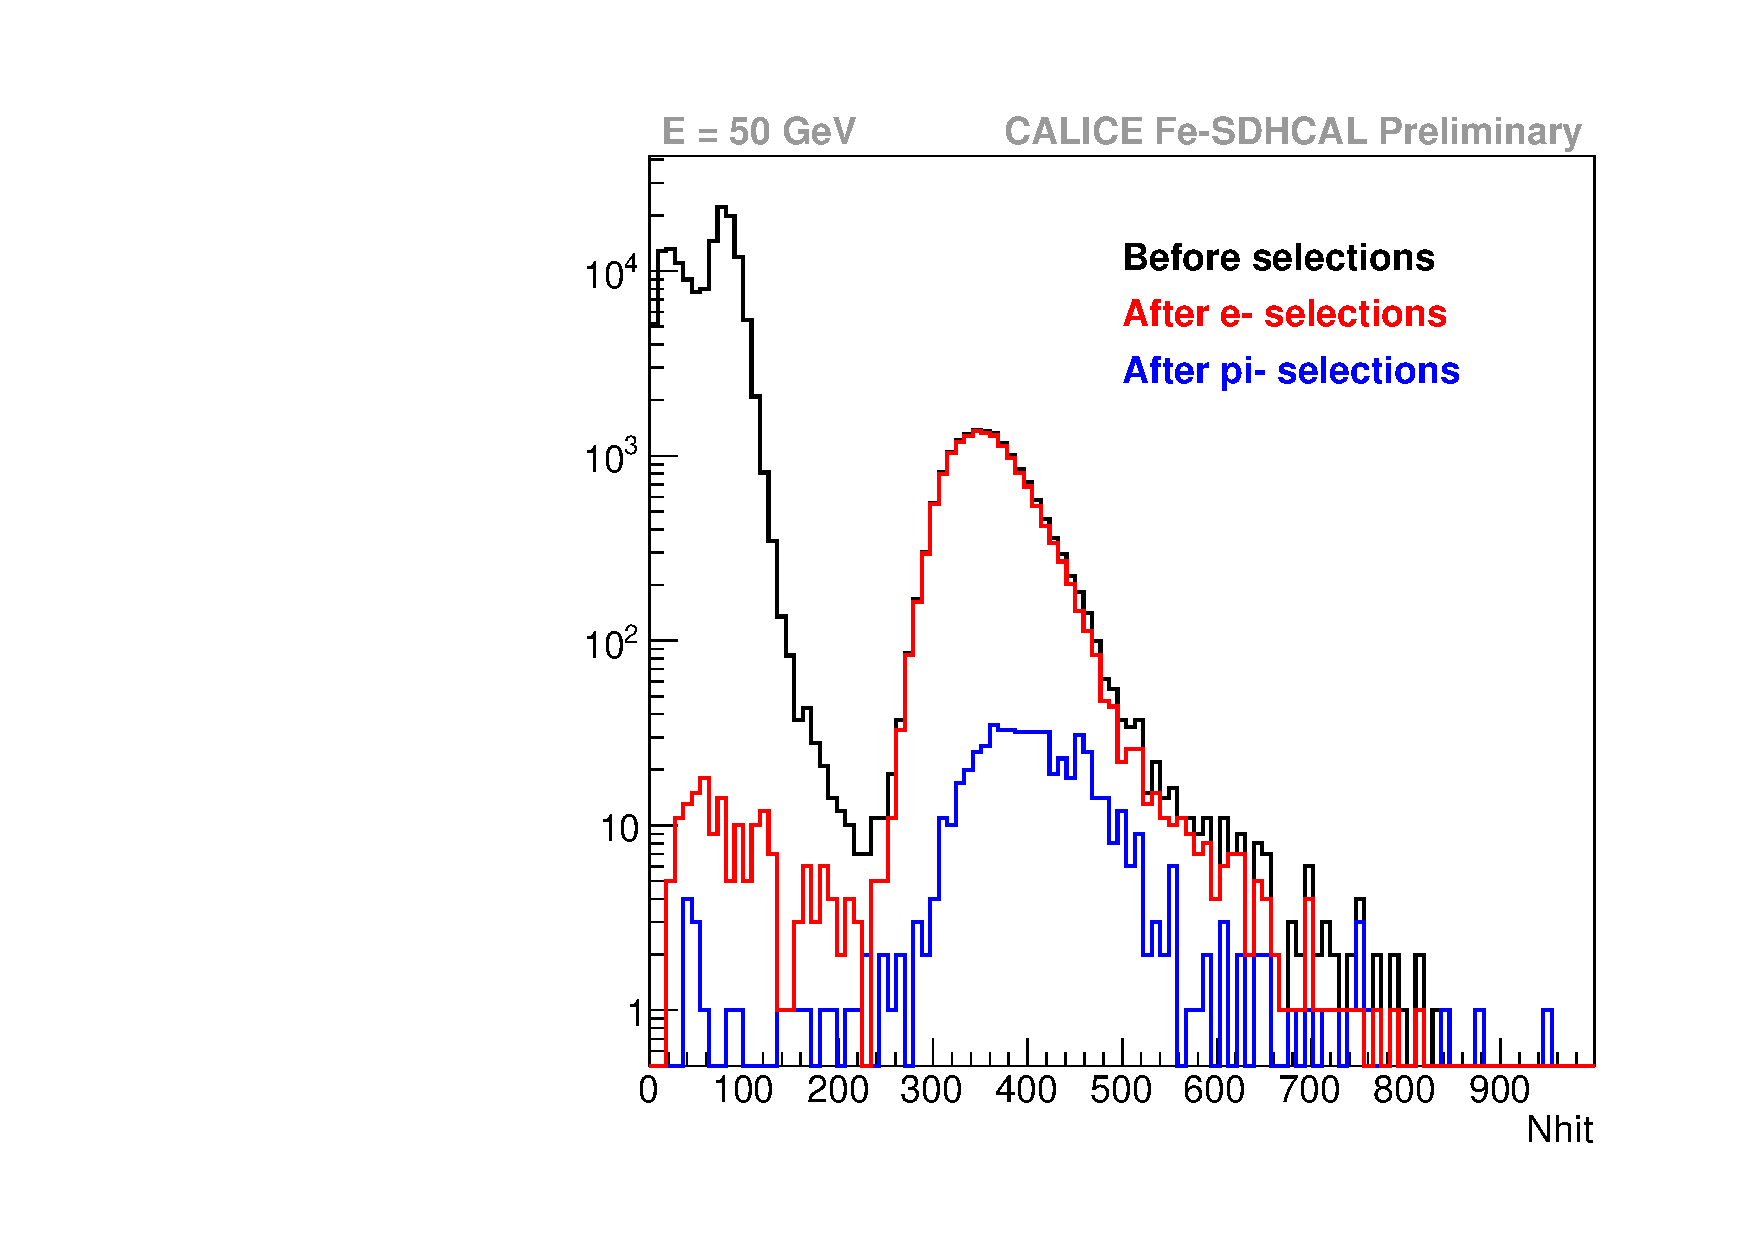
\includegraphics[width=.5\textwidth]{Digitizer/figs/selection715716.pdf}}
  \caption{Distribution du nombre de hits pour des échantillons de données d'électrons à 10 GeV (a) et 50 GeV (GeV). Les lignes noires montrent les distributions de nombres de hits avant les coupures, les lignes rouges après les coupures de sélection des électrons et les lignes bleu après les coupures de sélection des pions. \label{fig.e-Selection}}
\end{figure}

\begin{figure}[!ht]
  \begin{minipage}{.4\textwidth}
    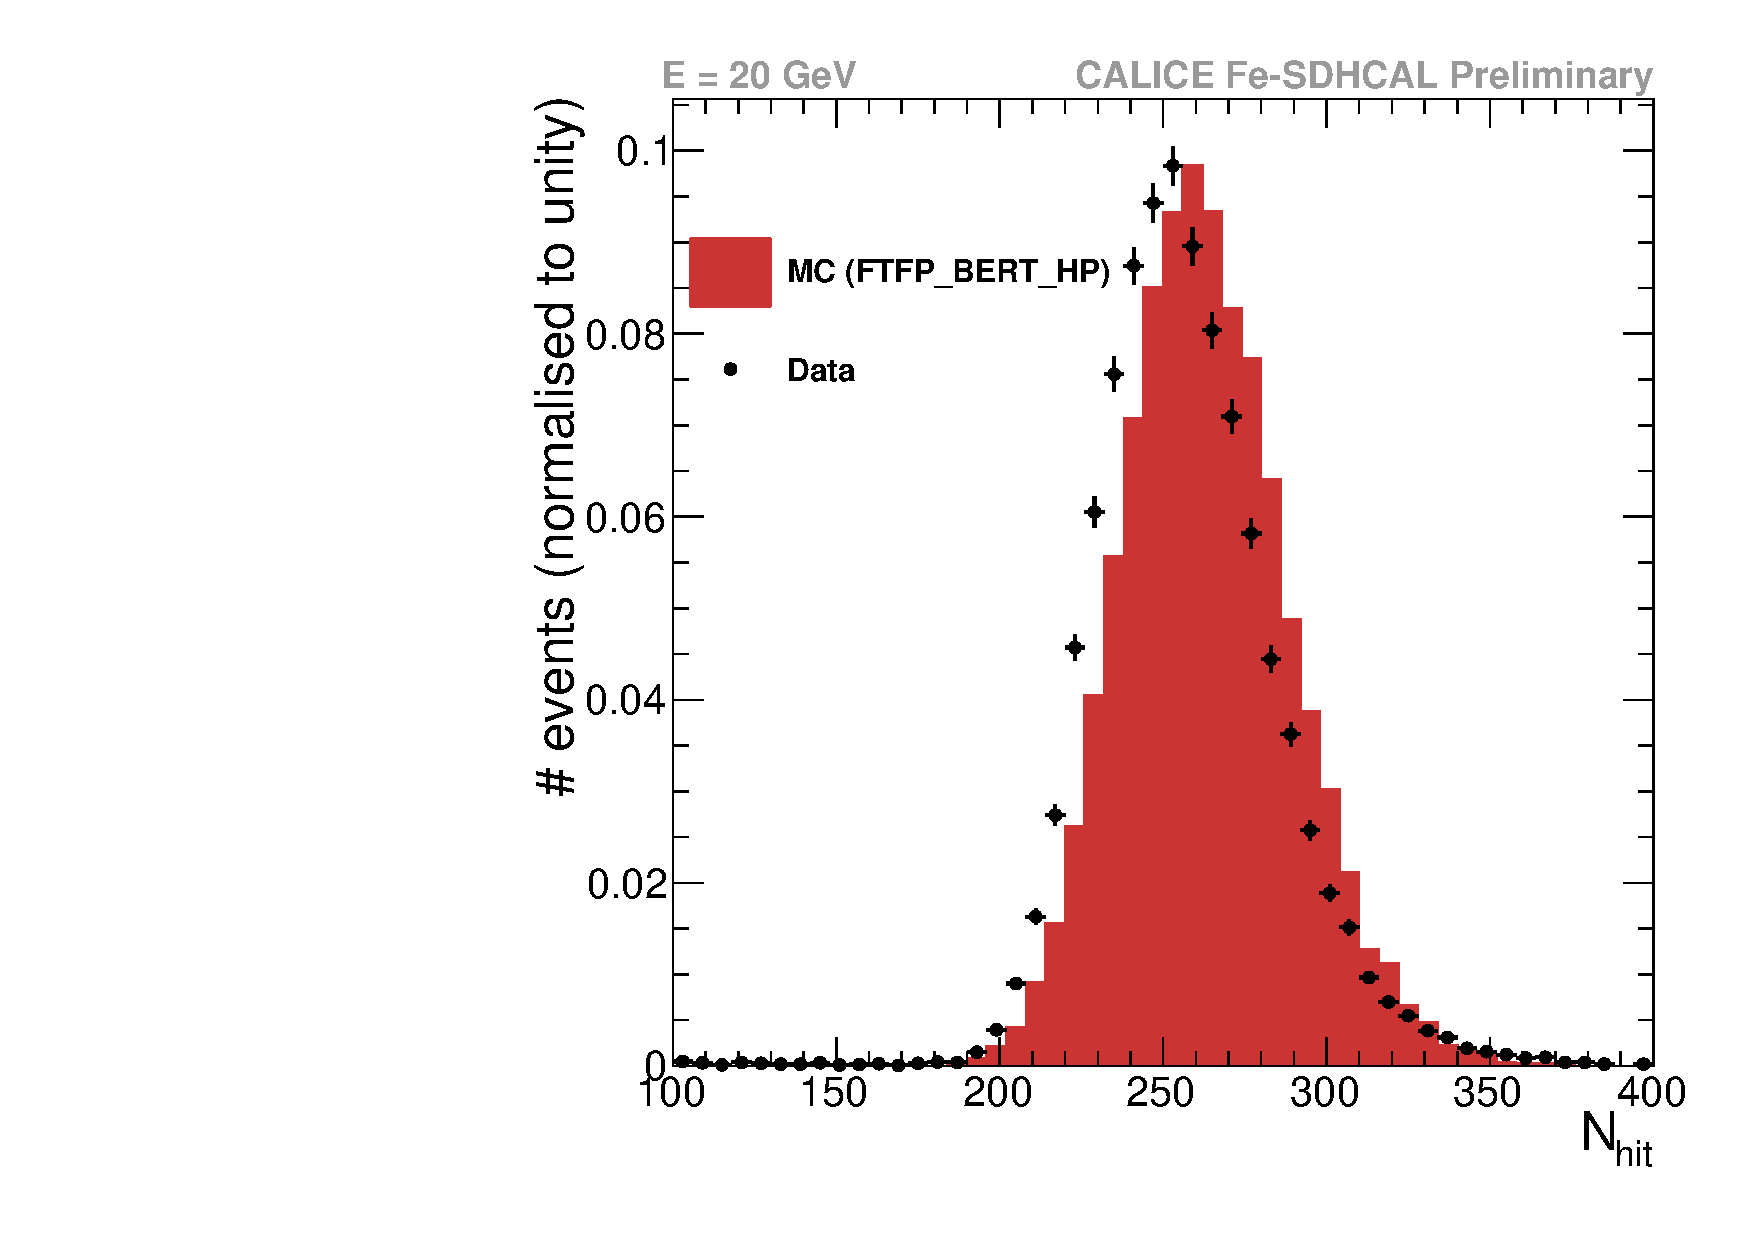
\includegraphics[width=1.0\textwidth]{Digitizer/figs/nhit_e-_20GeV_AugSep2012.pdf}\\
    \subfigure[]{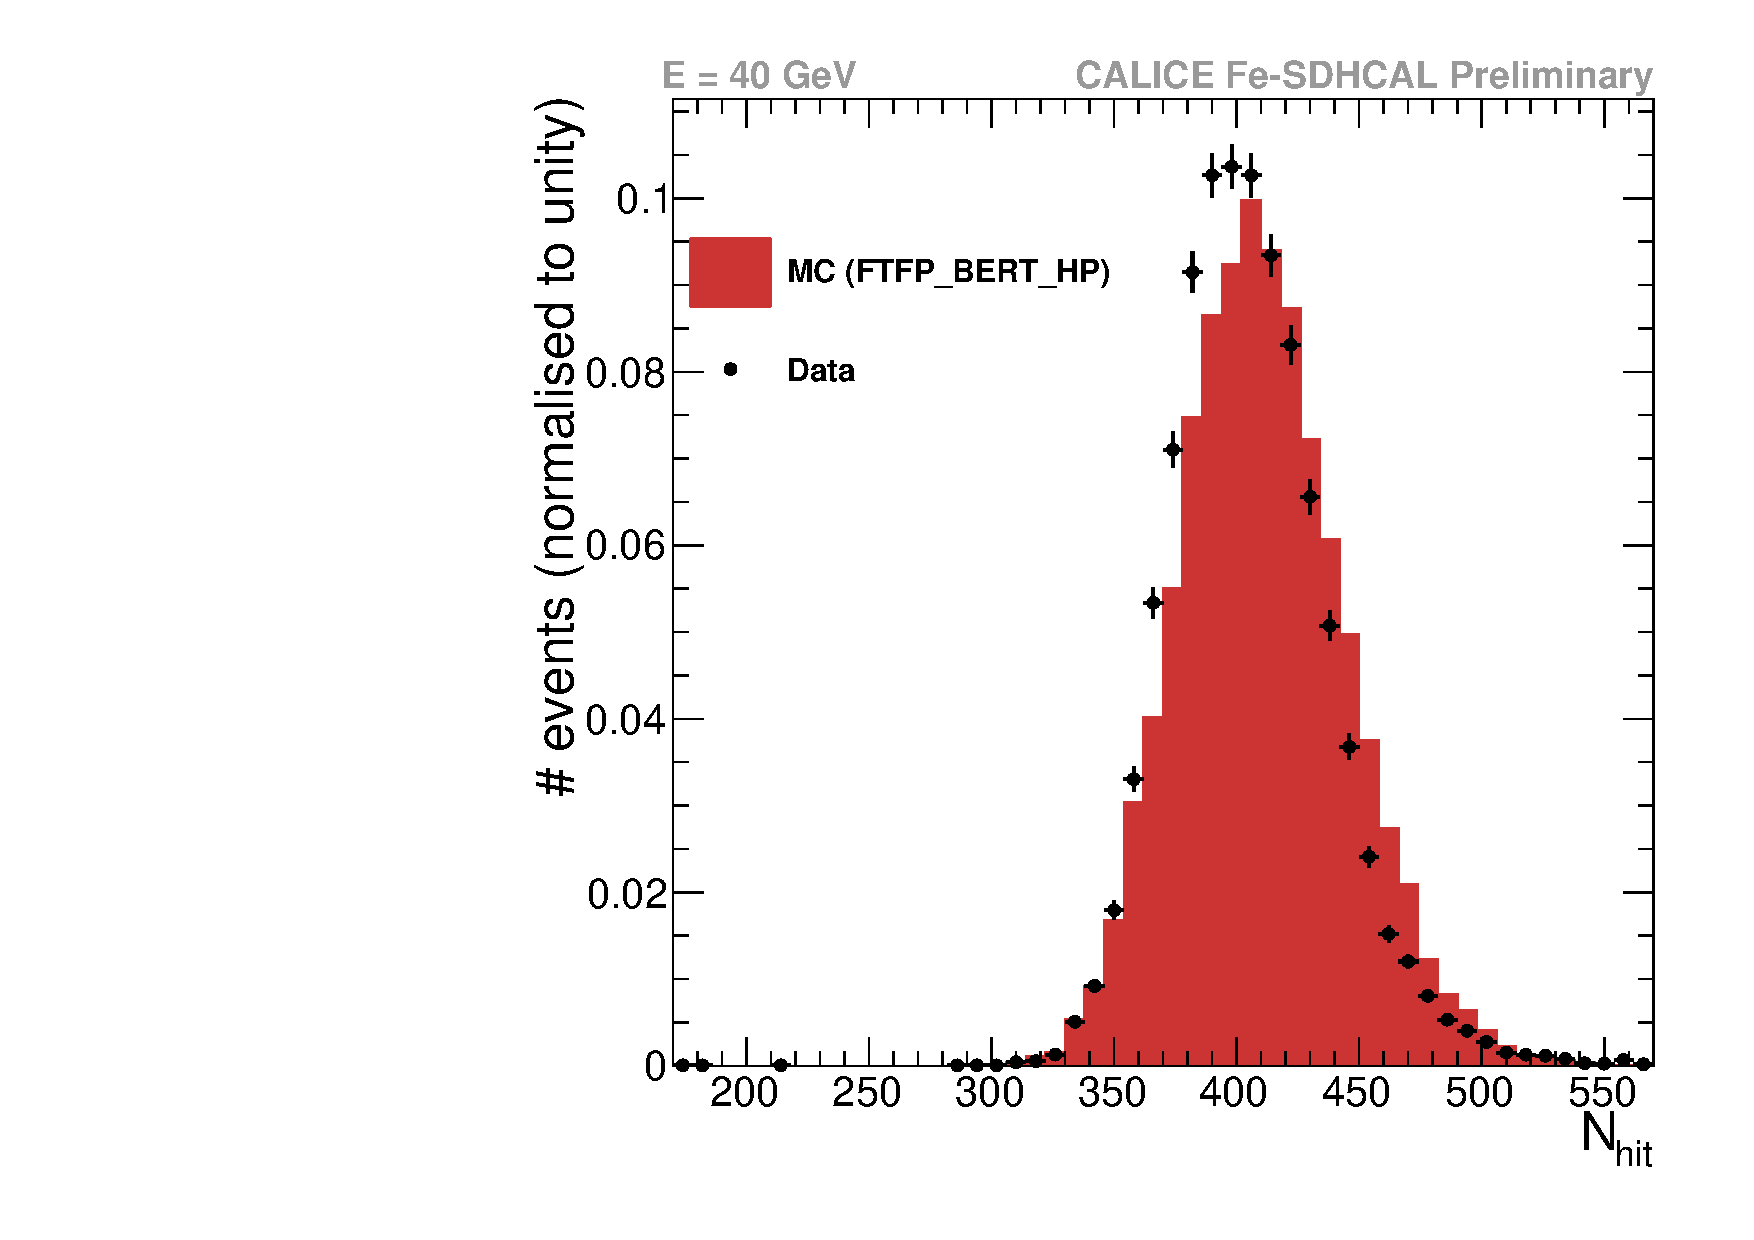
\includegraphics[width=1.0\textwidth]{Digitizer/figs/nhit_e-_40GeV_AugSep2012.pdf}}
  \end{minipage}
  \hfill
  \begin{minipage}{.6\textwidth}
    \subfigure[]{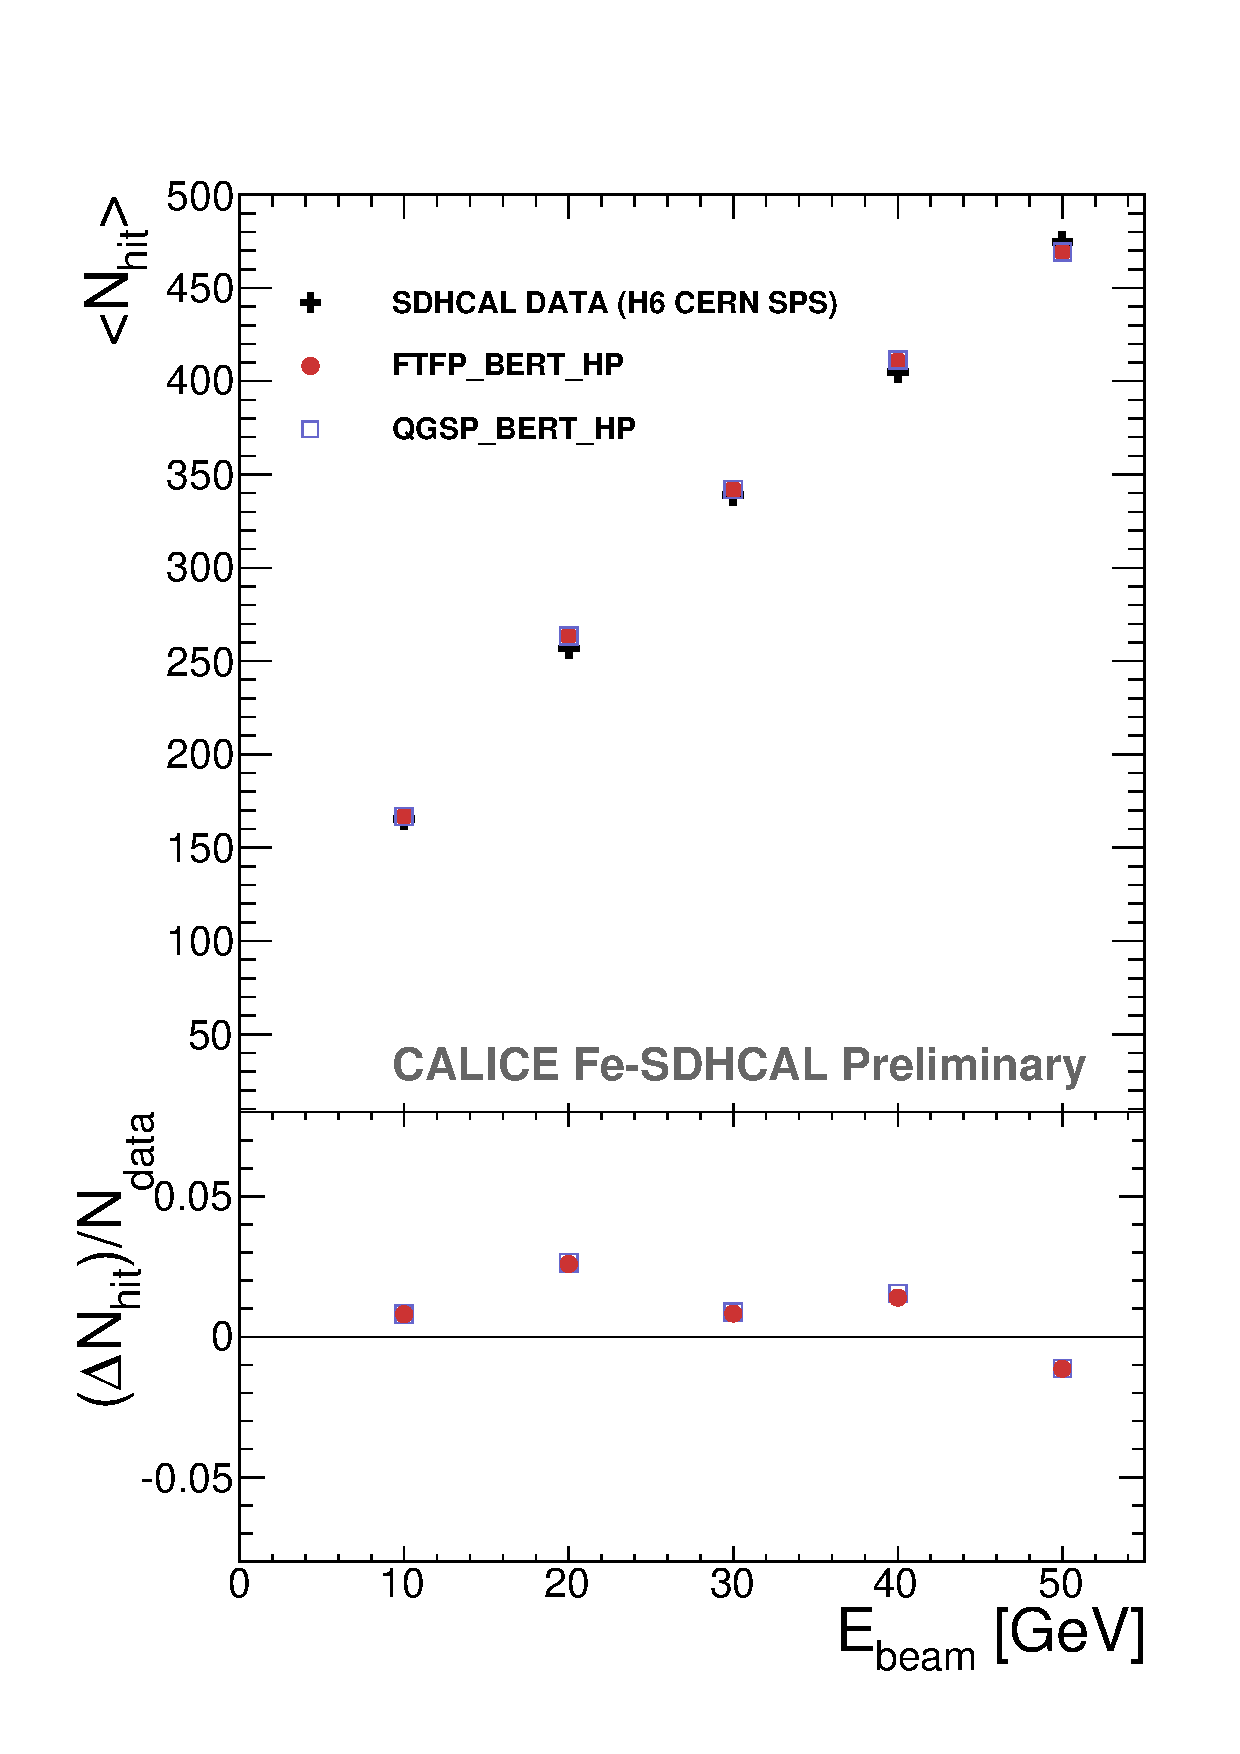
\includegraphics[width=1.0\textwidth]{Digitizer/figs/NHITELECTRON.pdf}}
  \end{minipage}
  \caption{(a) : Distribution de nombre de hits pour des échantillons d'électrons de 20 GeV (en haut) et 40 GeV (en bas). Les données sont représenté par des croix noires et la simulation par les histogrammes rouges. (b) : Moyenne du nombre de hits pour des échantillons d'électrons en focntion de l'énéergie du faisceau. Les données sont représentés par des croix noires et la simulation par des cerles rouges (FTFP\_BERT\_HP) et des carrés bleus (QGSP\_BERT\_HP). La déviation relative est aussi présentée.}
  \label{fig.nhite-}
\end{figure}

%%%%%%%%%%%%%%%%%%%%%

\subsubsection{Gerbes hadroniques}

\begin{figure}[!ht]
  \subfigure[]{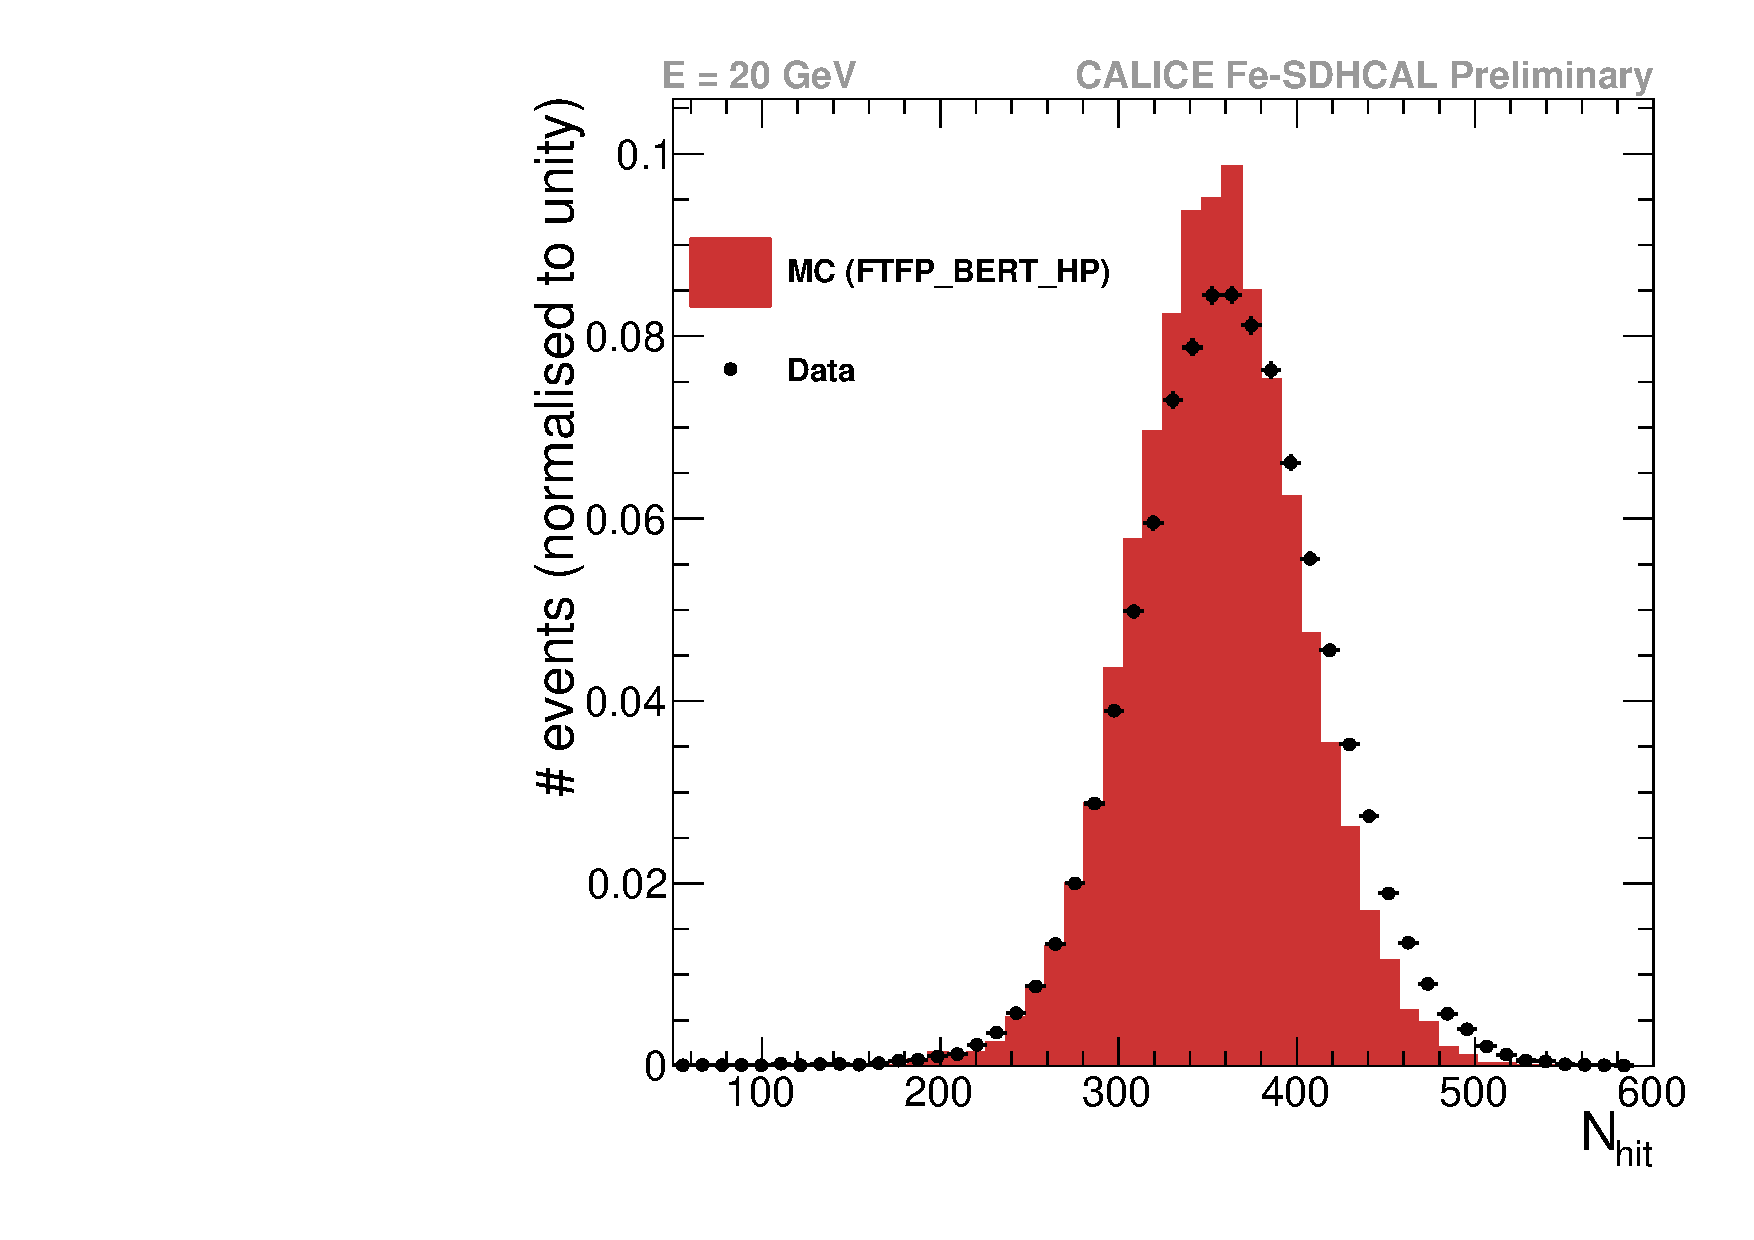
\includegraphics[width=.5\textwidth]{Digitizer/figs/nhit_pi-_20GeV_AugSep2012.pdf}}
  \subfigure[]{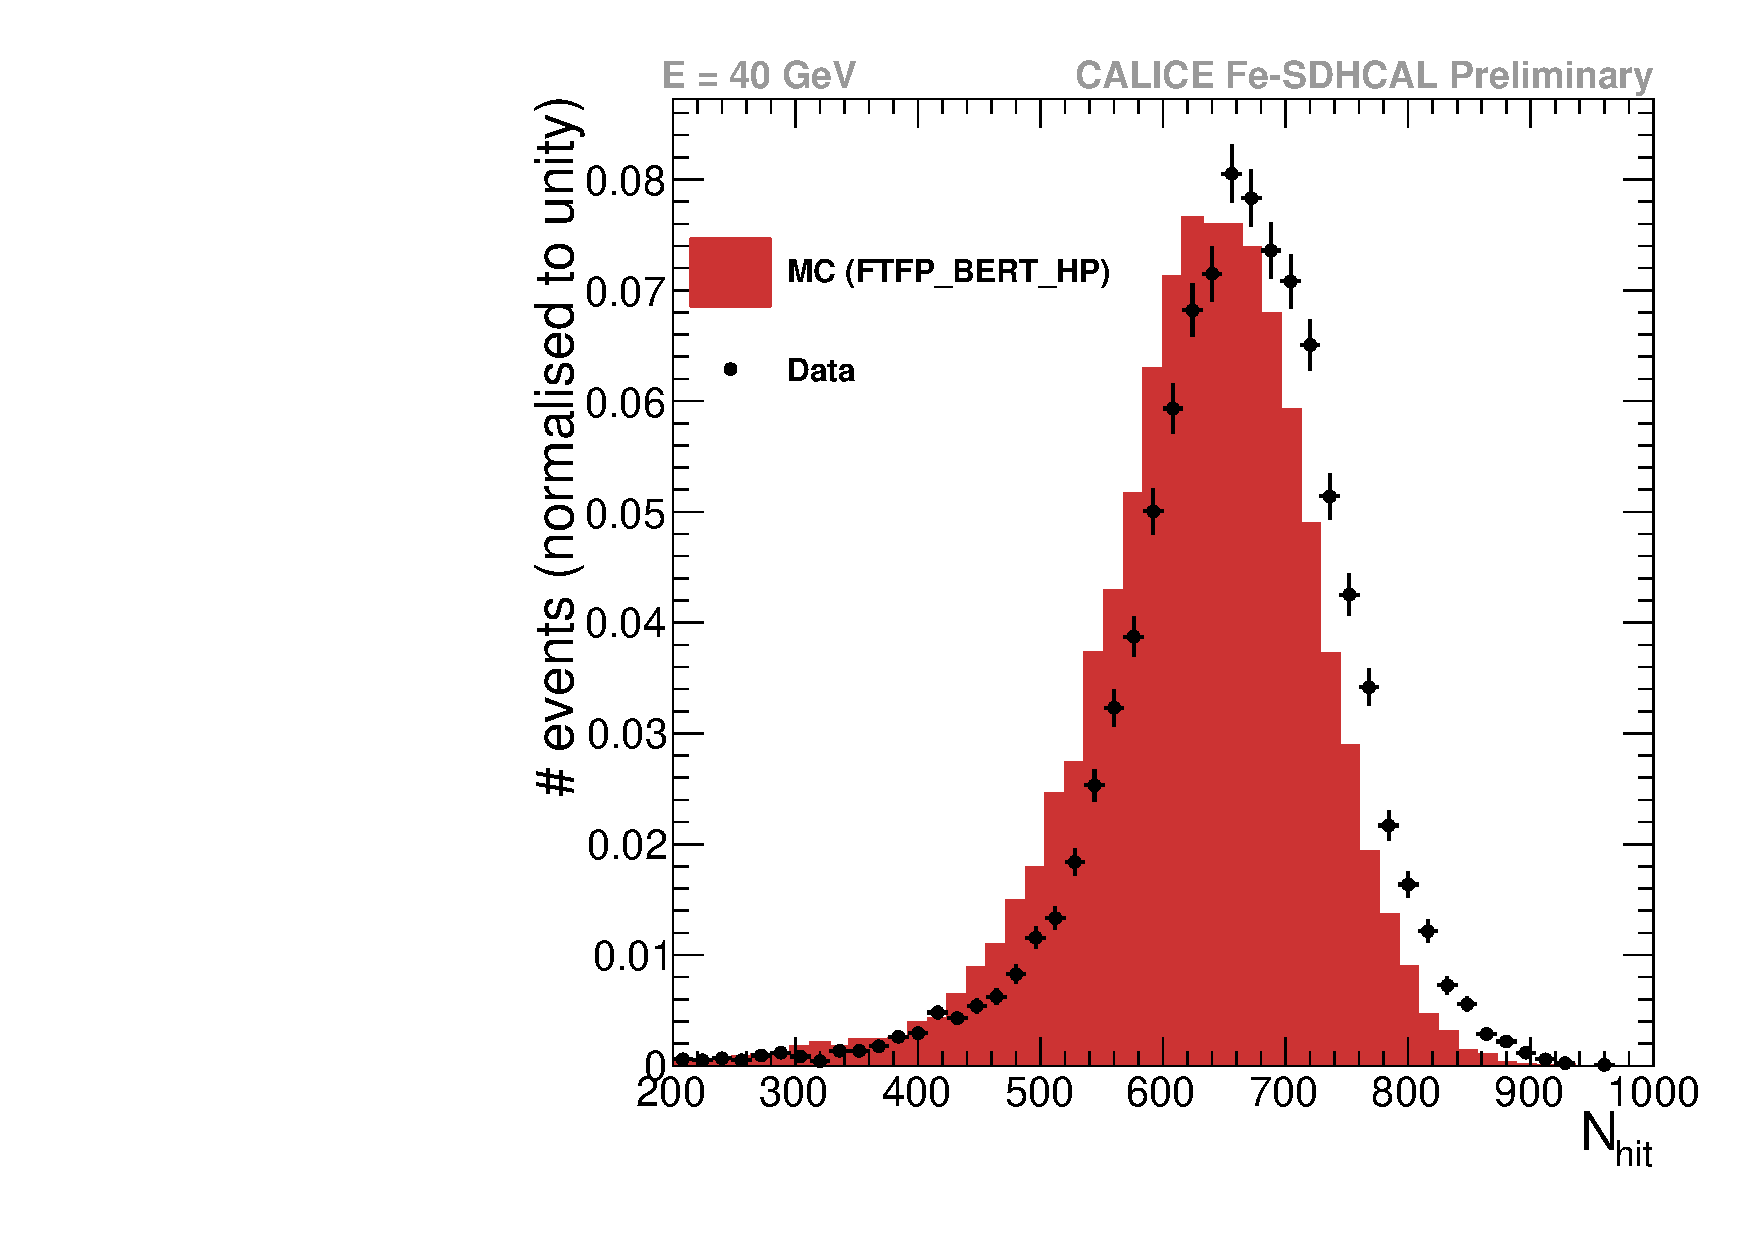
\includegraphics[width=.5\textwidth]{Digitizer/figs/nhit_pi-_40GeV_AugSep2012.pdf}}
  \subfigure[]{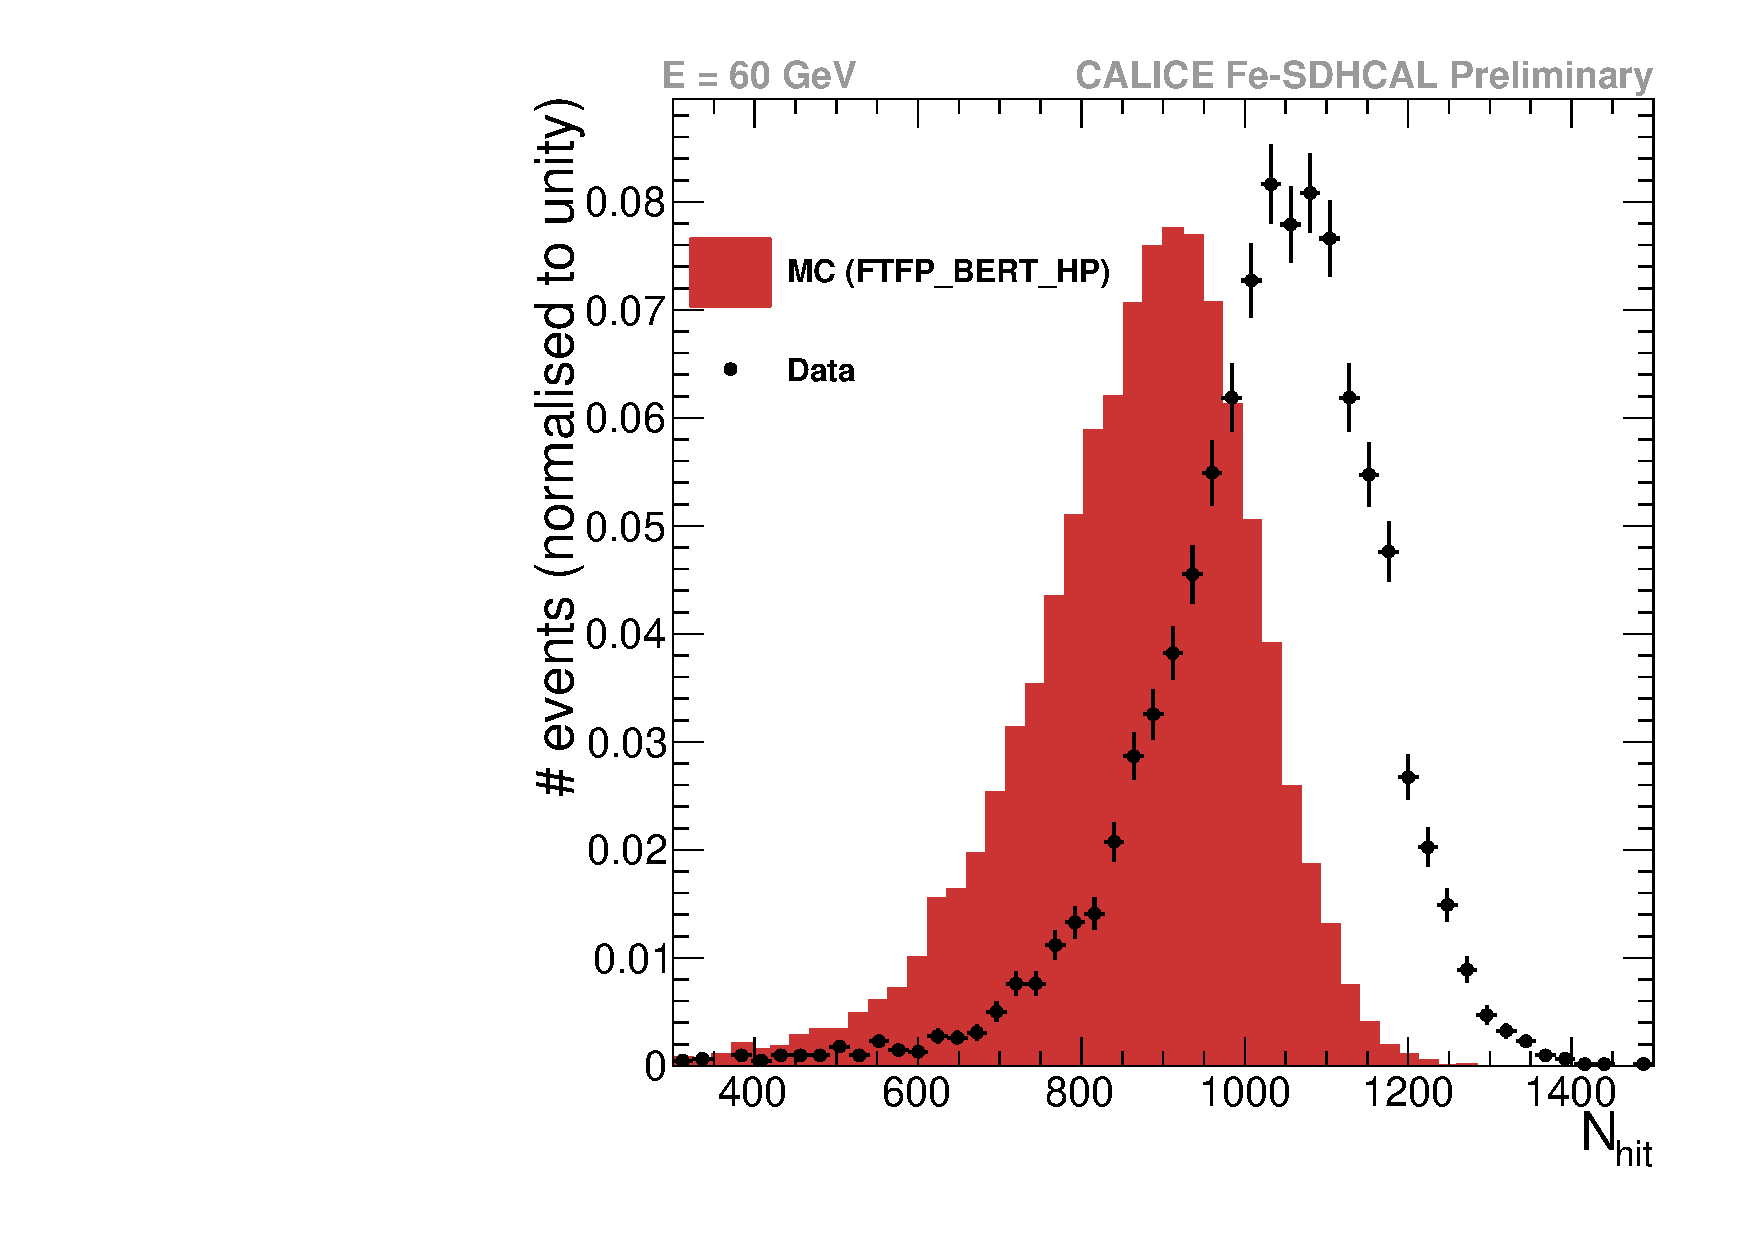
\includegraphics[width=.5\textwidth]{Digitizer/figs/nhit_pi-_60GeV_AugSep2012.pdf}}
  \subfigure[]{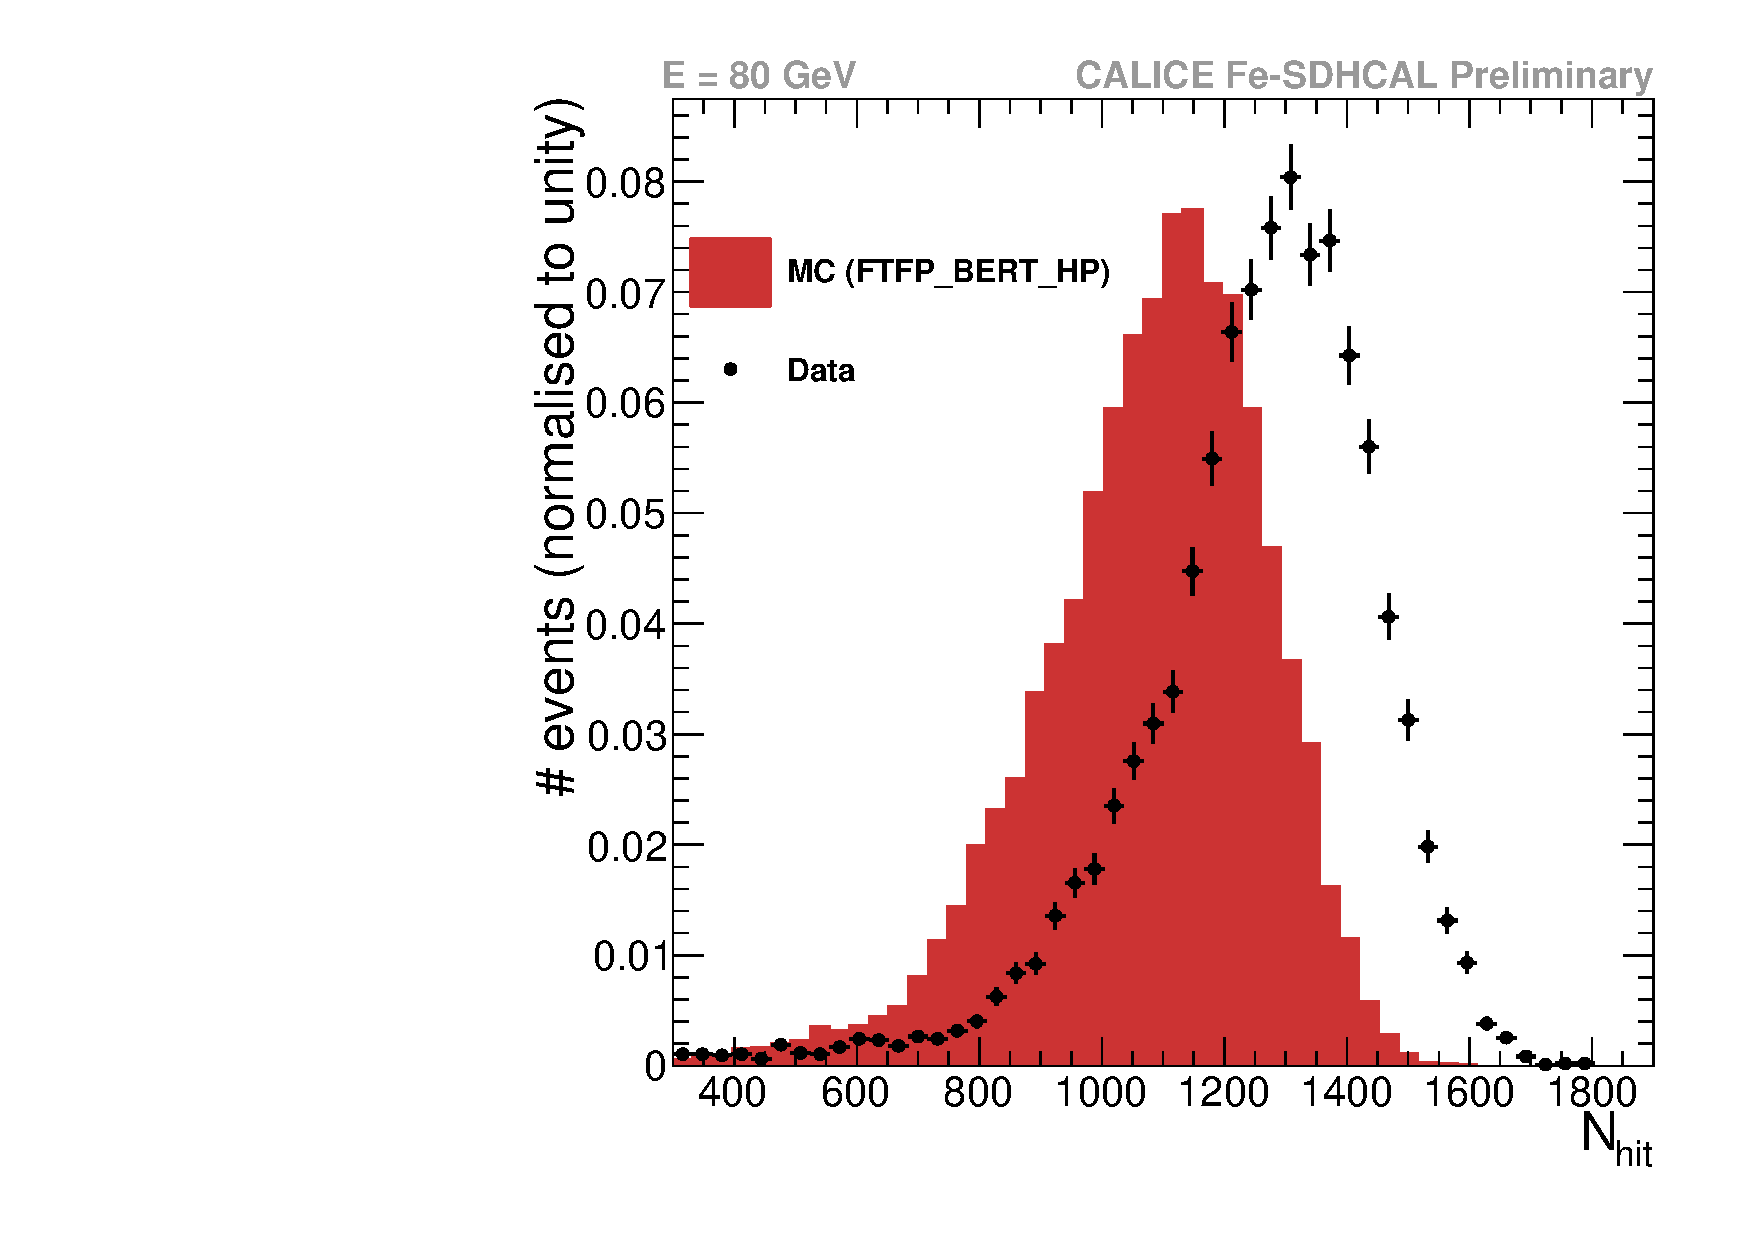
\includegraphics[width=.5\textwidth]{Digitizer/figs/nhit_pi-_80GeV_AugSep2012.pdf}}
  \caption{Distribution du nombre de hits pour des échantillons de pions de 20 GeV (a), de 40 GeV(b), de 60 GeV (c) et de 80 GeV (d). Les données sont représentées par des croix noires et la simulation par les histogrammes rouges.\label{fig.pi-nhit}}
\end{figure}

\begin{figure}[!ht]
  \subfigure[]{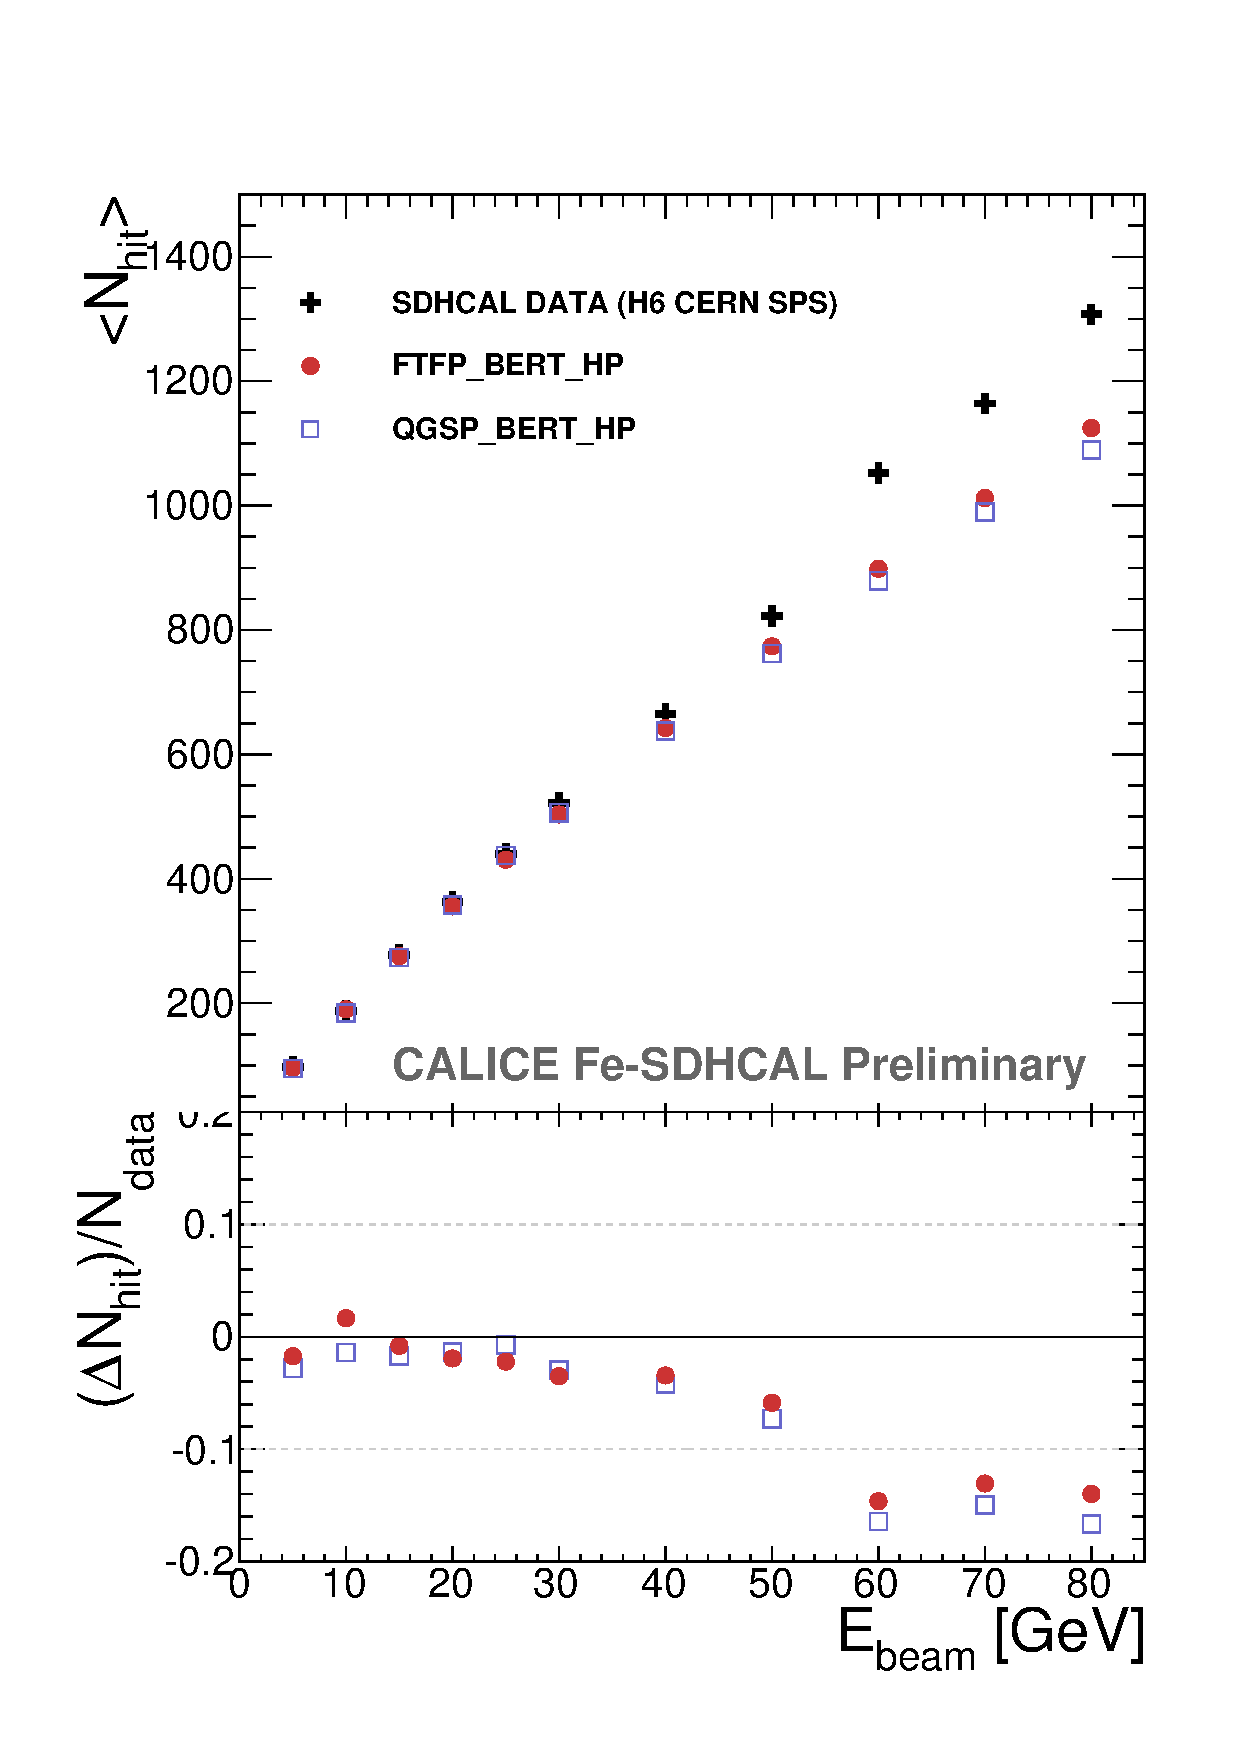
\includegraphics[width=.5\textwidth]{Digitizer/figs/NHITPION.pdf}}
  \subfigure[]{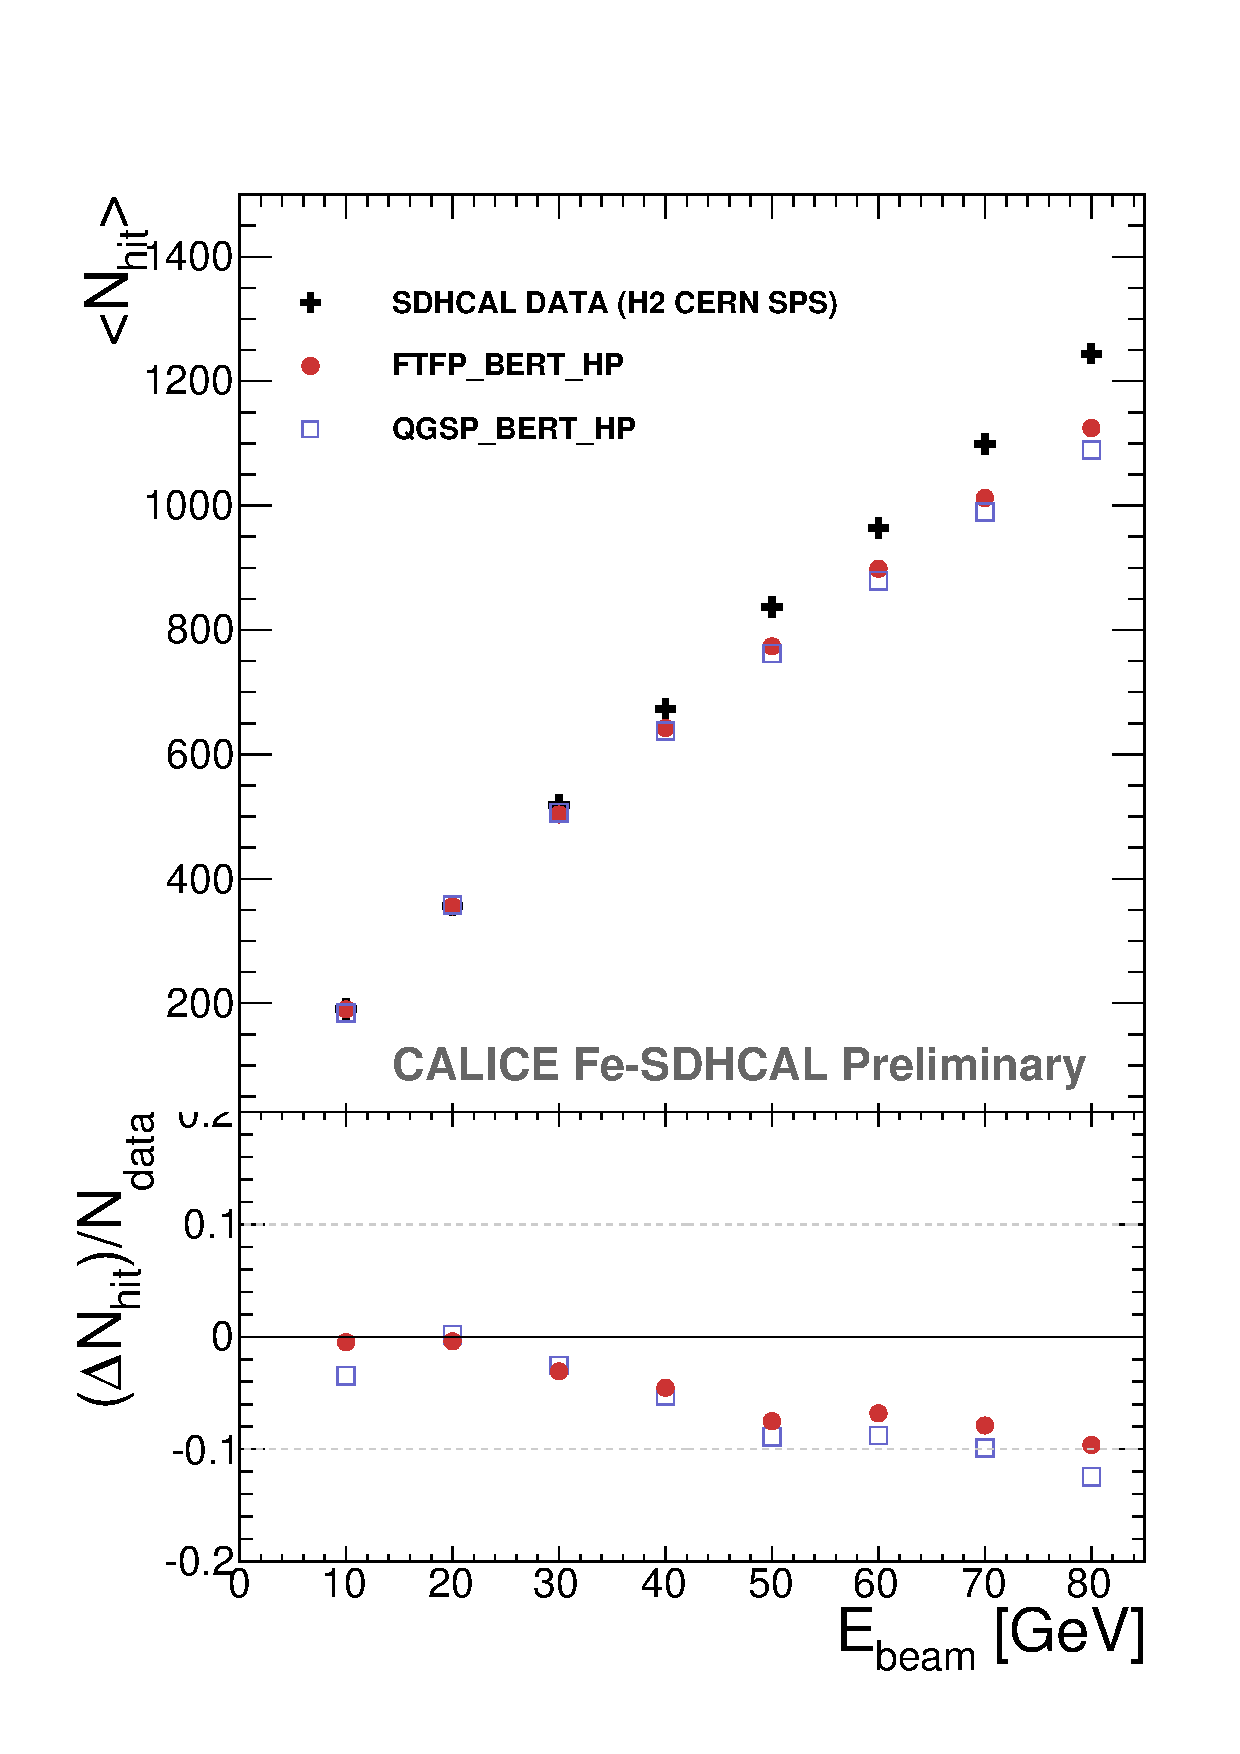
\includegraphics[width=.5\textwidth]{Digitizer/figs/NHITPIONNOV.pdf}}
  \caption{Moyenne du nombre de hits for des échantillons de pions en fonction de l'énergie du faisceau. Les données sont représentés par des croix noires et la simulation par des cerles rouges (FTFP\_BERT\_HP) et des carrés bleus (QGSP\_BERT\_HP). La déviation relative est aussi présentée. (a) : données enregistrées sur la ligne H6 du SPS au CERN; (b) : données enregistrées sur la ligne H2 du SPS au CERN.}
  \label{fig.nhit_pi-_ebeam}
\end{figure}

%%%%%%%%%%%%%%%%%%%%%%%%%%%%%%%%%%%%%%%%%%%%%%%

\section{Conclusion}
